\documentclass[11pt,table]{beamer}
%\documentclass[11pt,handout]{beamer}
\mode<presentation>
\usepackage{etex}
\usepackage{graphicx}
\usepackage{epstopdf}
\usepackage[english]{babel}
\usepackage{tabularx}
\usepackage{booktabs}
\usepackage{mathrsfs}
\usepackage{multicol}
\usepackage{bm}
\usepackage{subcaption}
\usepackage{wrapfig}
\usepackage{dcolumn}
\usepackage{threeparttable}
\usepackage{booktabs}
\usepackage{bbm}
\usepackage{amsmath,dsfont,listings}
\usepackage{amssymb}
\usepackage{rotating}
\usepackage{multirow}
\usepackage[authoryear]{natbib}
\usepackage{circledsteps}
\usepackage{tikz}
\usetikzlibrary{arrows,decorations.pathmorphing,backgrounds,fit,positioning,shapes.symbols,chains}
\setbeamertemplate{section in toc}[sections numbered]
\setbeamertemplate{caption}[numbered]

\bibliographystyle{Econometrica}

\setbeamersize{text margin right=3.5mm, text margin left=7.5mm}  % text margin
\setbeamersize{sidebar width left=0cm, sidebar width right=0mm}
\setbeamertemplate{sidebar right}{}
\setbeamertemplate{sidebar left}{}

\definecolor{text-grey}{rgb}{0.45, 0.45, 0.45} % grey text on white background
\definecolor{bg-grey}{rgb}{0.66, 0.65, 0.60} % grey background (for white text)
\definecolor{fu-blue}{RGB}{0, 51, 102} % blue text
\definecolor{fu-green}{RGB}{153, 204, 0} % green text
\definecolor{fu-red}{RGB}{204, 0, 0} % red text (used by \alert)

\setbeamertemplate{frametitle}{%
    \vskip-30pt \color{text-grey}\large%
    \begin{minipage}[b][23pt]{80.5mm}%
    \flushleft\insertframetitle%
    \end{minipage}%
}

\setbeamertemplate{navigation symbols}{} 

%%% begin title page
\setbeamertemplate{title page}{
\vskip2pt\hfill
\vskip6pt\hskip3pt

% set the title and the author
\vskip14pt
\parbox[top][1.35cm][c]{11cm}{\LARGE\color{text-grey}\inserttitle \\[1ex] \small \insertsubtitle \\[3ex]}
\vskip11pt
\parbox[top][1.35cm][c]{11cm}{\small \insertauthor \; \insertinstitute \\[2ex] \insertdate}
}
%%% end title page

%%% colors
\usecolortheme{lily}
\setbeamercolor*{normal text}{fg=black,bg=white}
\setbeamercolor*{alerted text}{fg=fu-red}
\setbeamercolor*{example text}{fg=fu-green}
\setbeamercolor*{structure}{fg=fu-blue}

\setbeamercolor*{block title}{fg=white,bg=black!50}
\setbeamercolor*{block title alerted}{fg=white,bg=black!50}
\setbeamercolor*{block title example}{fg=white,bg=black!50}

\setbeamercolor*{block body}{bg=black!10}
\setbeamercolor*{block body alerted}{bg=black!10}
\setbeamercolor*{block body example}{bg=black!10}

\setbeamercolor{bibliography entry author}{fg=fu-blue}
\setbeamercolor{bibliography entry journal}{fg=text-grey}
\setbeamercolor{item}{fg=fu-blue}
\setbeamercolor{navigation symbols}{fg=text-grey,bg=bg-grey}
%%% end colors

%%% headline
\setbeamertemplate{headline}{
\vskip30pt
}
%%% end headline

%%% footline
\newcommand{\footlinetext}{
%\insertshortinstitute, \insertshorttitle, \insertshortdate
}
\setbeamertemplate{footline}{
\vskip2pt
\hfill \raisebox{-1pt}{\usebeamertemplate***{navigation symbols}}
\hfill \insertframenumber\hspace{10pt}
\vskip4pt
}
%%% end footline

%%% settings for listings package
\lstset{extendedchars=true, showstringspaces=false, basicstyle=\footnotesize\sffamily, tabsize=2, breaklines=true, breakindent=10pt, frame=l, columns=fullflexible}
\lstset{language=Java} % this sets the syntax highlighting
\lstset{mathescape=true} % this switches on $...$ substitution in code
% enables UTF-8 in source code:
\lstset{literate={�}{{\"a}}1 {�}{{\"o}}1 {�}{{\"u}}1 {�}{{\"A}}1 {�}{{\"O}}1 {�}{{\"U}}1 {�}{\ss}1}
%%% end listings

\usepackage{concmath}
\usepackage{xcolor}
\definecolor{lightblue}{rgb}{0.8,0.85,1}
\definecolor{persianred}{rgb}{0.8, 0.2, 0.2}
\definecolor{red1}{RGB}{206, 17, 38}
\definecolor{blue1}{RGB}{16, 118, 208}
\definecolor{gray1}{RGB}{117, 115, 115}
\usepackage{hyperref}
\hypersetup{
    bookmarks=false,
    unicode=false,
    pdftoolbar=false,
    pdffitwindow=true,
    pdftitle={Econometricks: Short guides to econometrics},
    pdfauthor={Davud Rostam-Afschar},
    pdfsubject={econometrics},
    pdfcreator={Davud Rostam-Afschar},
    pdfproducer={Davud Rostam-Afschar},
    pdfkeywords={econometrics},
    pdfnewwindow=true,
}

\def\beX{\begin{itemize}}
\def\beXX{\begin{itemize}}
\def\beXXX{\begin{itemize}}
\def\beXXXX{\begin{itemize}}
\def\eeX{\end{itemize}}
\def\eeXX{\end{itemize}}
\def\eeXXX{\end{itemize}}
\def\eeXXXX{\end{itemize}}
\newtheorem{proposition}{Proposition}
\newtheorem{assumption}{Definition}

\title[] 
{Econome\textcolor{red1}{tricks}: Short guides to econometrics\\[1ex]\normalsize 
}

\author[D. Rostam-Afschar]{Trick 04: The Least Squares Estimator\\[2ex]}

\institute[]{\textcolor{gray1}{Davud Rostam-Afschar (Uni Mannheim)}}
            
\date[] 
{}

\subject{Econometrics}
\renewcommand{\footlinetext}{\insertshortinstitute, \insertshorttitle, \insertshortdate}

\def\sym#1{\ifmmode^{#1}\else\(^{#1}\)\fi}

\begin{document}

\begin{frame}[plain]
  \titlepage
\end{frame}

% --------------------------------------------------- Slide --
\begin{frame}
	\frametitle{Content}
	\tableofcontents[]
\end{frame}



\section{What is the Relationship between Two Variables?}

% --------------------------------------------------- Slide --
\begin{frame}
	\frametitle{Content}
	\tableofcontents[%
 		currentsection, % causes all sections but the current to be shown in a semi-transparent way.
 		%currentsubsection, % causes all subsections but the current subsection in the current section to ...
 		%hideallsubsections, % causes all subsections to be hidden.
 		%hideothersubsections, % causes the subsections of sections other than the current one to be hidden.
 		%part=, % part number causes the table of contents of part part number to be shown
 		%pausesections, % causes a \pause command to be issued before each section. This is useful if you
 		%pausesubsections, %  causes a \pause command to be issued before each subsection.
 		%sections={ overlay specification },
	]

\end{frame}

\begin{frame}{Political Connections and Firms}
\beamerdefaultoverlayspecification{<+->}
Firm profits increase with the degree of political connections
\begin{figure}[t]
	\centering
		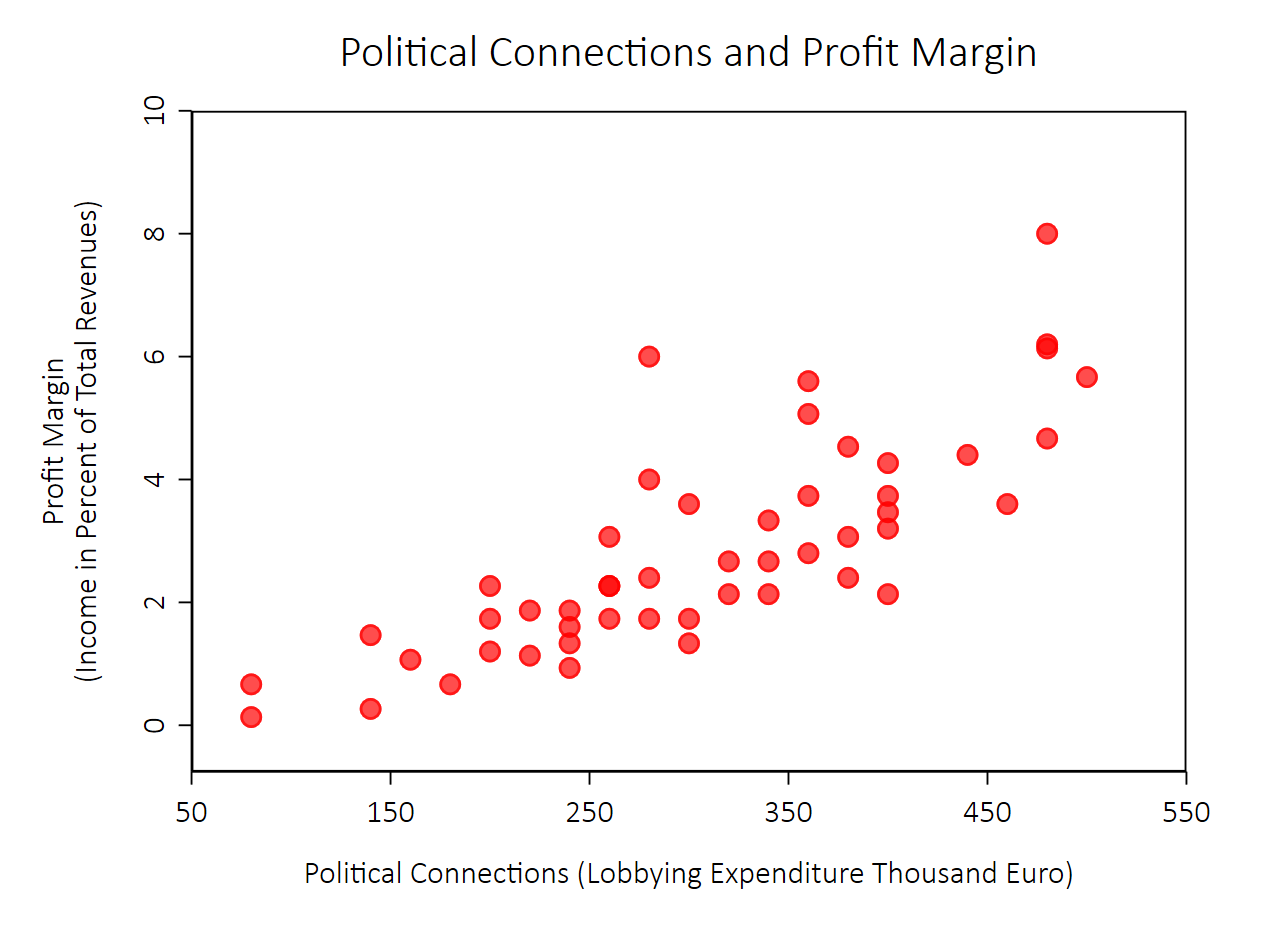
\includegraphics[height=.50\textheight]{figures/politicallyconnected1}
   \label{fig:politicallyconnected1}
\end{figure}
\pause
\begin{itemize}
	\item Learn how to represent relationships between two or more variables
	\item How to quantify and predict effects of shocks and policy changes
	\item Show properties of the OLS estimator in small \& large samples
	\item Apply Monte Carlo Simulations to assess properties of OLS

\end{itemize}
\end{frame}

\section{The Econometric Model}

% --------------------------------------------------- Slide --
\begin{frame}
	\frametitle{Content}
	\tableofcontents[%
 		currentsection, % causes all sections but the current to be shown in a semi-transparent way.
 		%currentsubsection, % causes all subsections but the current subsection in the current section to ...
 		%hideallsubsections, % causes all subsections to be hidden.
 		%hideothersubsections, % causes the subsections of sections other than the current one to be hidden.
 		%part=, % part number causes the table of contents of part part number to be shown
 		%pausesections, % causes a \pause command to be issued before each section. This is useful if you
 		%pausesubsections, %  causes a \pause command to be issued before each subsection.
 		%sections={ overlay specification },
	]

\end{frame}

\begin{frame}{Specification of a Linear Regression}
%\beamerdefaultoverlayspecification{<+->}


\begin{columns}
\begin{column}{0.45\textwidth}
\small
\begin{itemize}
	\item dependent variable\\
	$y_i = $ profits of firm $i$
	\item explanatory variables\\
	$x_{i1}, \ldots, x_{iK}$ $k=1,\ldots K$\\
	political connections, other firm characteristics
	\item $x_{i0} = 1$ is a constant
	\item parameters to be estimated\\
	$\beta_0, \beta_1, \ldots, \beta_K$ are $K+1$
	\item $u_i$ is called the error term
\end{itemize} 
\end{column}
\begin{column}{0.55\textwidth}  %%<--- here
    \begin{center}
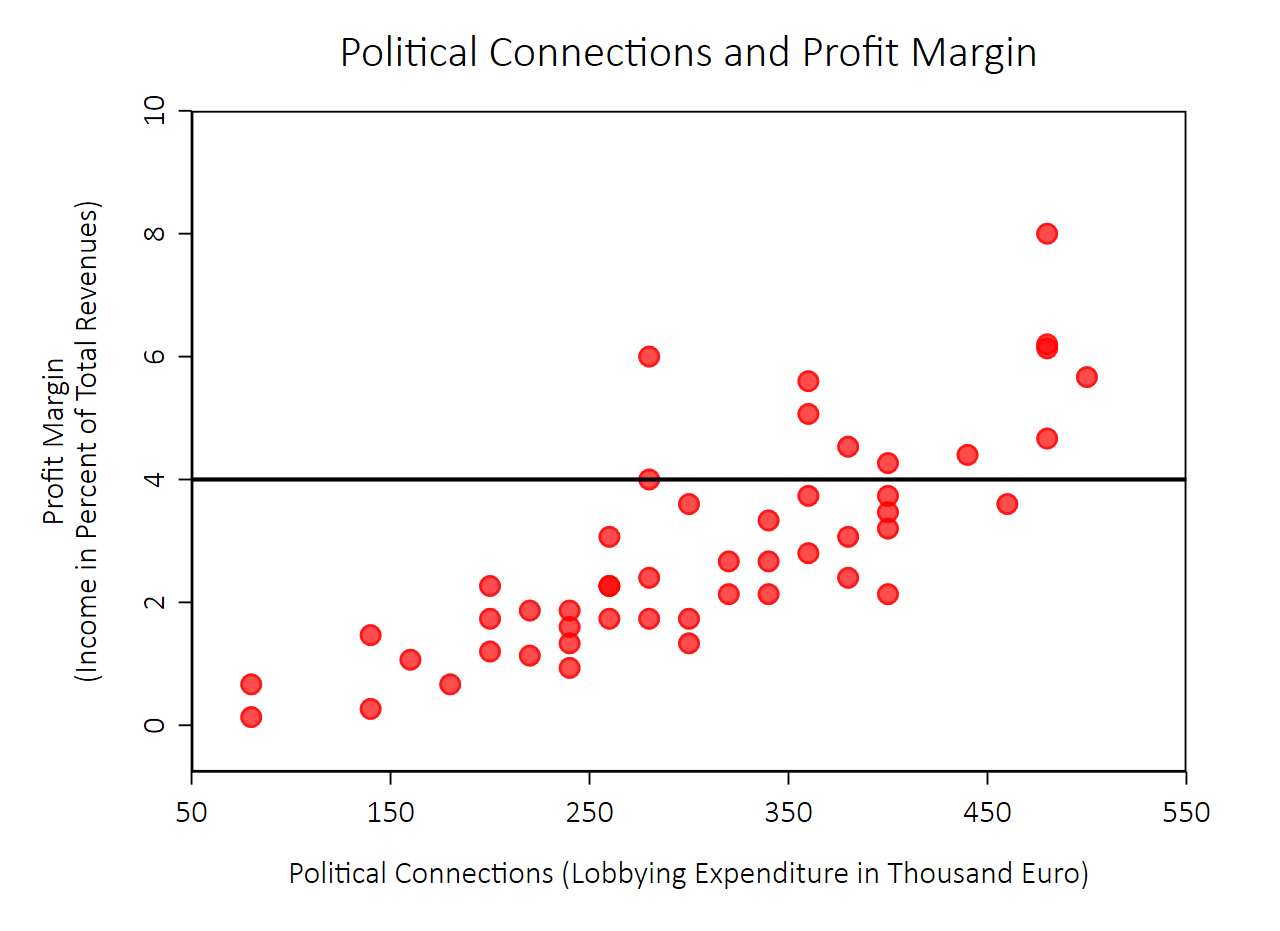
\includegraphics[width=1\textwidth]{figures/politicallyconnected2}
     \end{center}

\end{column}
\end{columns}
\quad\\[2ex]
$$y_i = (\beta_0=4) + (\beta_1=0) x_{i1} + u_{i}.$$


\end{frame}


\begin{frame}{Specification of a Linear Regression}
%\beamerdefaultoverlayspecification{<+->}


\begin{columns}
\begin{column}{0.45\textwidth}
\small
\begin{itemize}
	\item dependent variable\\
	$y_i = $ profits of firm $i$
	\item explanatory variables\\
	$x_{i1}, \ldots, x_{iK}$ $k=1,\ldots K$\\
	political connections, other firm characteristics
	\item $x_{i0} = 1$ is a constant
	\item parameters to be estimated\\
	$\beta_0, \beta_1, \ldots, \beta_K$ are $K+1$
	\item $u_i$ is called the error term\\[2ex]
\end{itemize} 

\end{column}
\begin{column}{0.55\textwidth}  %%<--- here
    \begin{center}
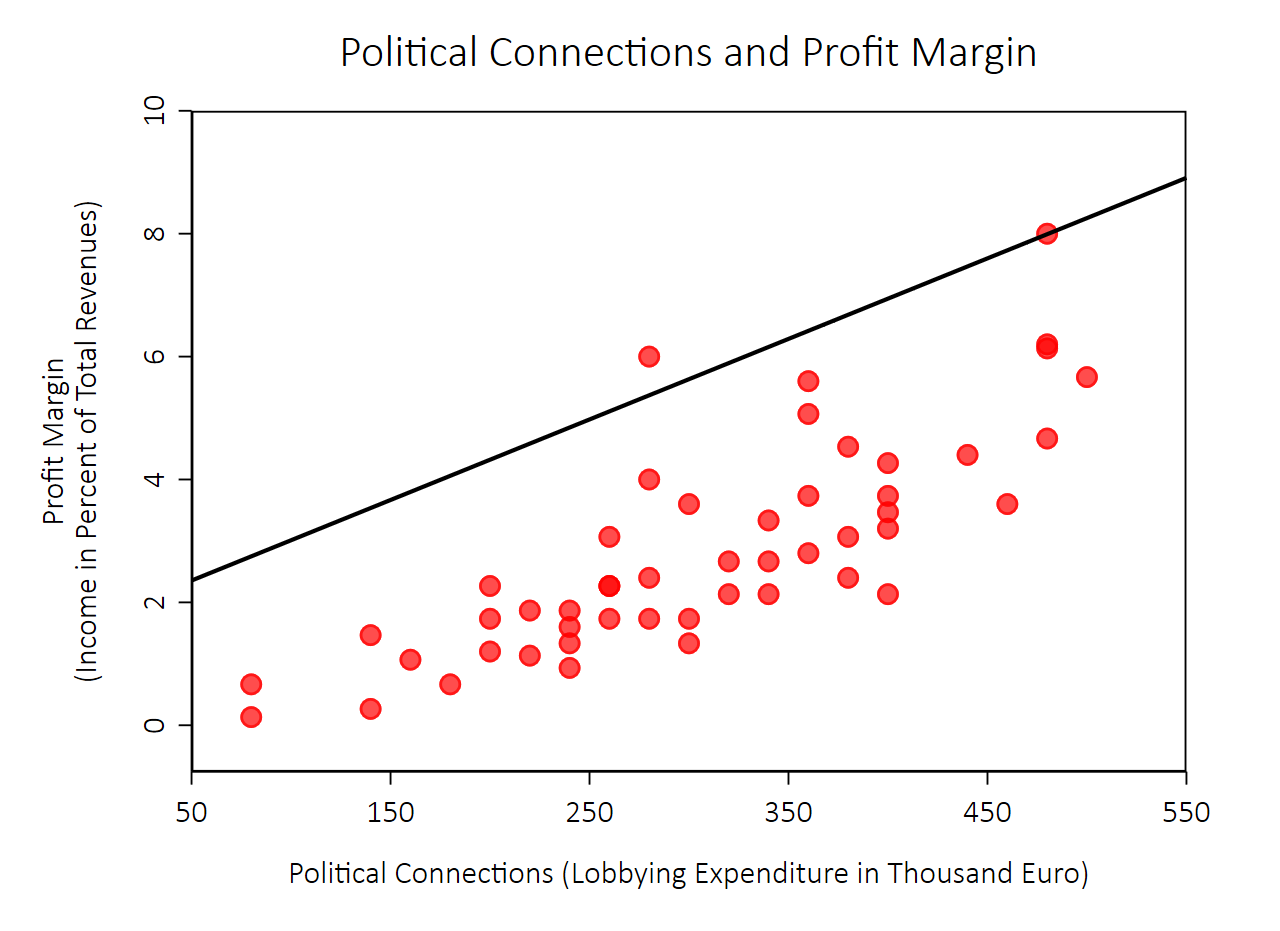
\includegraphics[width=1\textwidth]{figures/politicallyconnected3}
     \end{center}

\end{column}
			 

\end{columns}
\quad\\[2ex]
$$y_i = (\beta_0=2.36) + (\beta_1=0.01) x_{i1} + u_{i}.$$

\end{frame}


\begin{frame}{How Were the Data Generated?}
\beamerdefaultoverlayspecification{<+->}
The \emph{data generating process} is fully described by a set of assumptions.\\[2ex]
\textbf{The Five Assumptions of the Econometric Model}\pause
\begin{itemize}
	\item LRM1: Linearity
	\item LRM2: Simple random sampling
	\item LRM3: Exogeneity
	\item LRM4: Error variance
	\item LRM5: Identifiability
\end{itemize}

\end{frame}


\begin{frame}{Data Generating Process: Linearity}
%\beamerdefaultoverlayspecification{<+->}

\begin{assumption} \textbf{LRM1: Linearity}. 
$$y_i = \beta_0 + \beta_1 x_{i1} + \ldots + \beta_K x_{iK} + u_{i} \text{ and } E(u_i)=0.$$\pause
\end{assumption}
LRM1 assumes that the 
\begin{itemize}
	\item functional relationship is linear in parameters $\beta_k$\pause
	\item error term $u_{i}$ enters additively\pause
	\item parameters $\beta_k$ are constant across individual firms $i$ and $j\neq i$.
\end{itemize}


\end{frame}

\begin{frame}{Anscombe's Quartet}
%\beamerdefaultoverlayspecification{<+->}

%-------------------------------------------
%\begin{landscape}
%\begin{figure*}
\begin{figure}[htbp]
	\begin{subfigure}[c]{0.30\textwidth}
 \centering
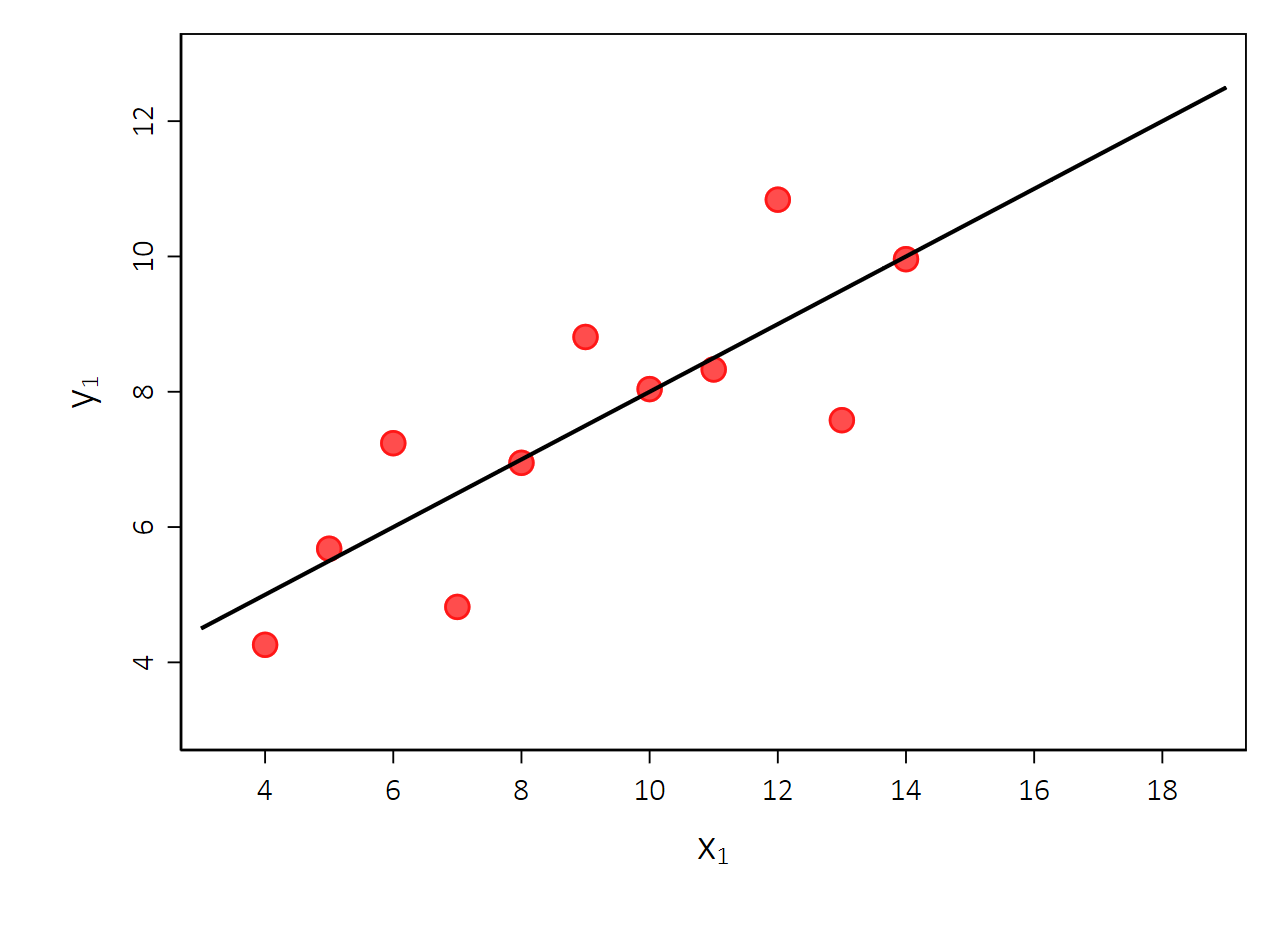
\includegraphics[width=1\textwidth]{figures/Anscombe_data1}
 						
  \end{subfigure}%
	\begin{subfigure}[c]{0.30\textwidth}
 \centering
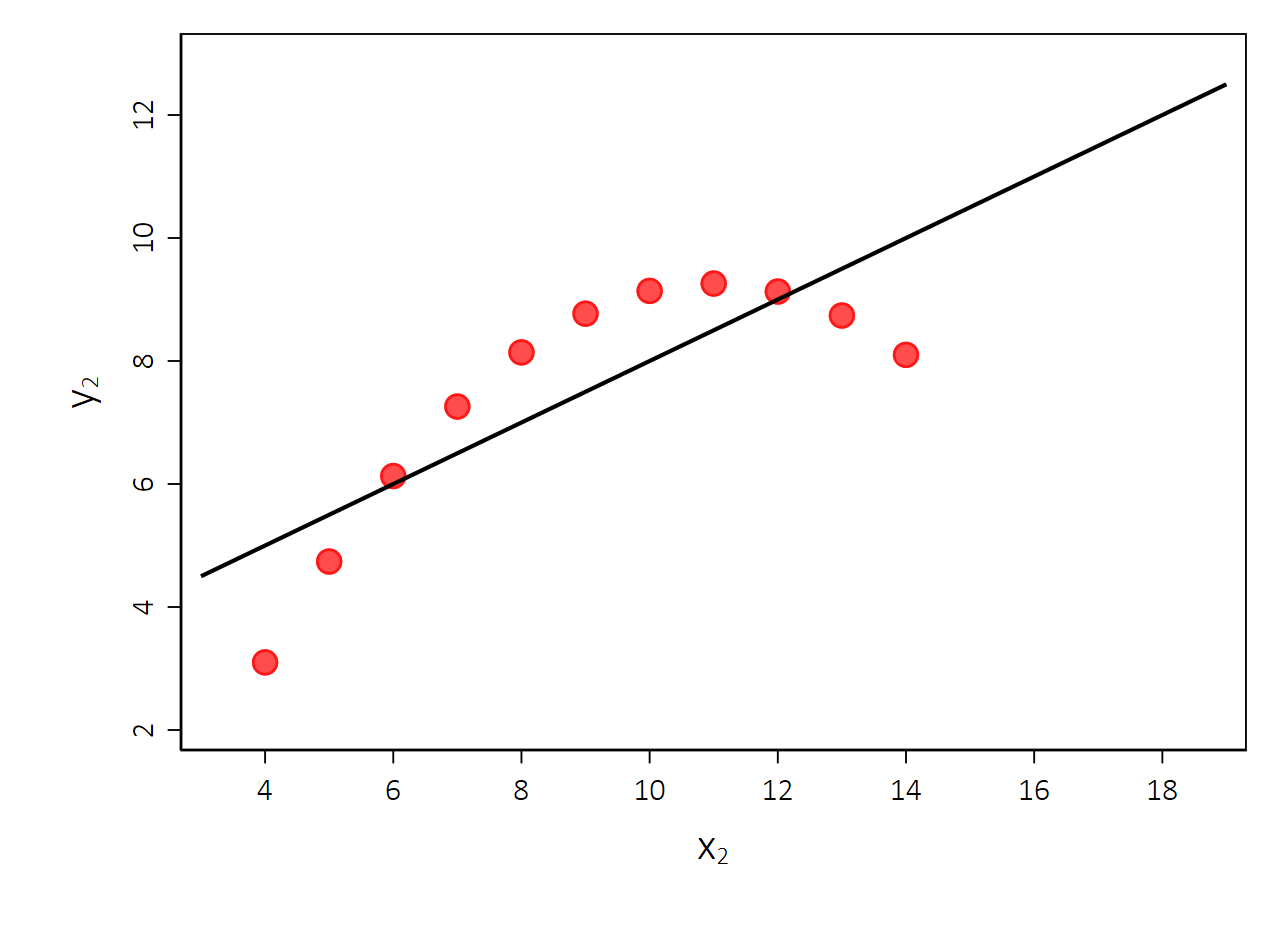
\includegraphics[width=1\textwidth]{figures/Anscombe_data2}
							
  \end{subfigure}\\
		\begin{subfigure}[c]{0.30\textwidth}
 \centering
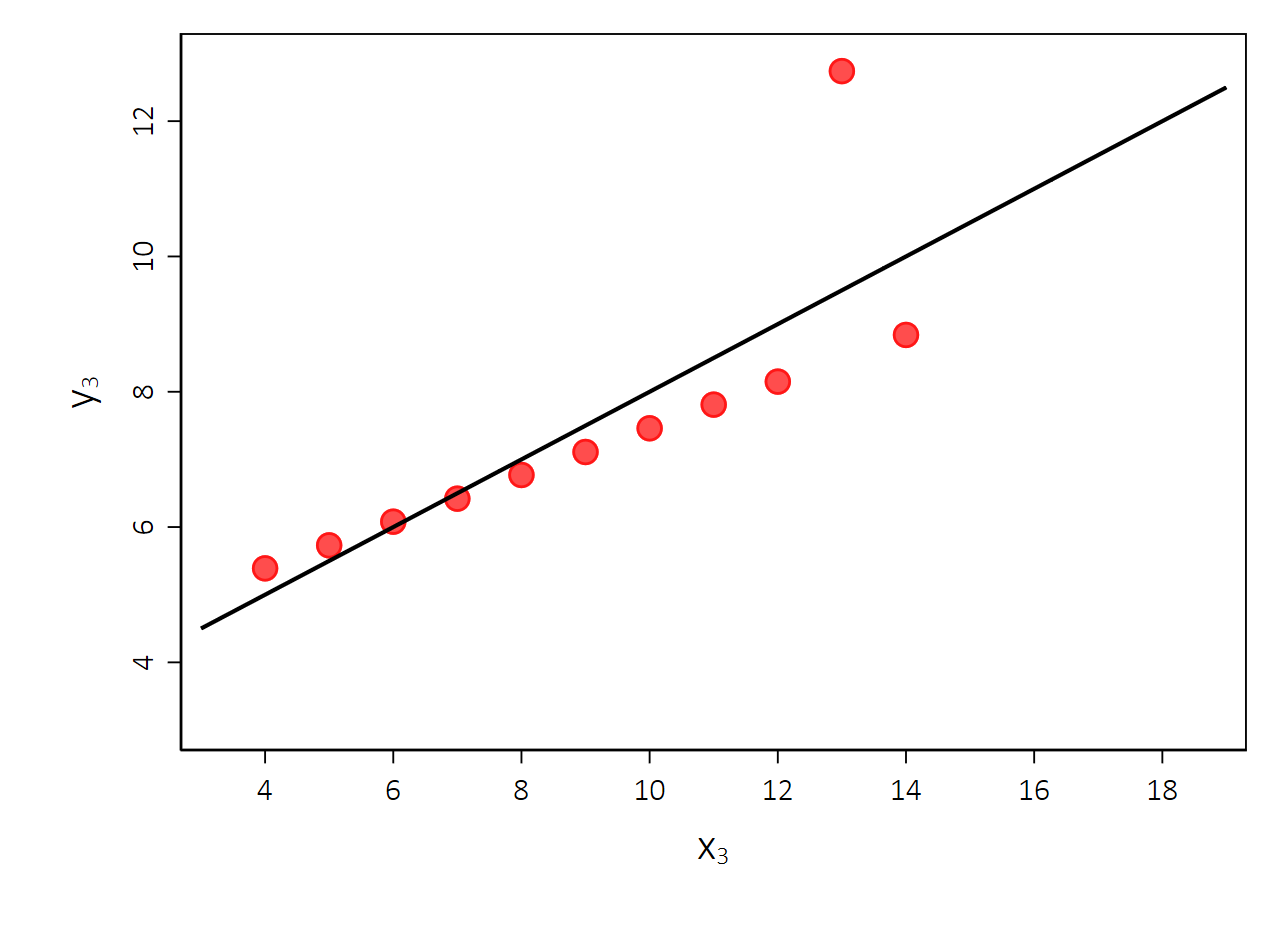
\includegraphics[width=1\textwidth]{figures/Anscombe_data3}
					
  \end{subfigure}%
	\begin{subfigure}[c]{0.30\textwidth}
 \centering
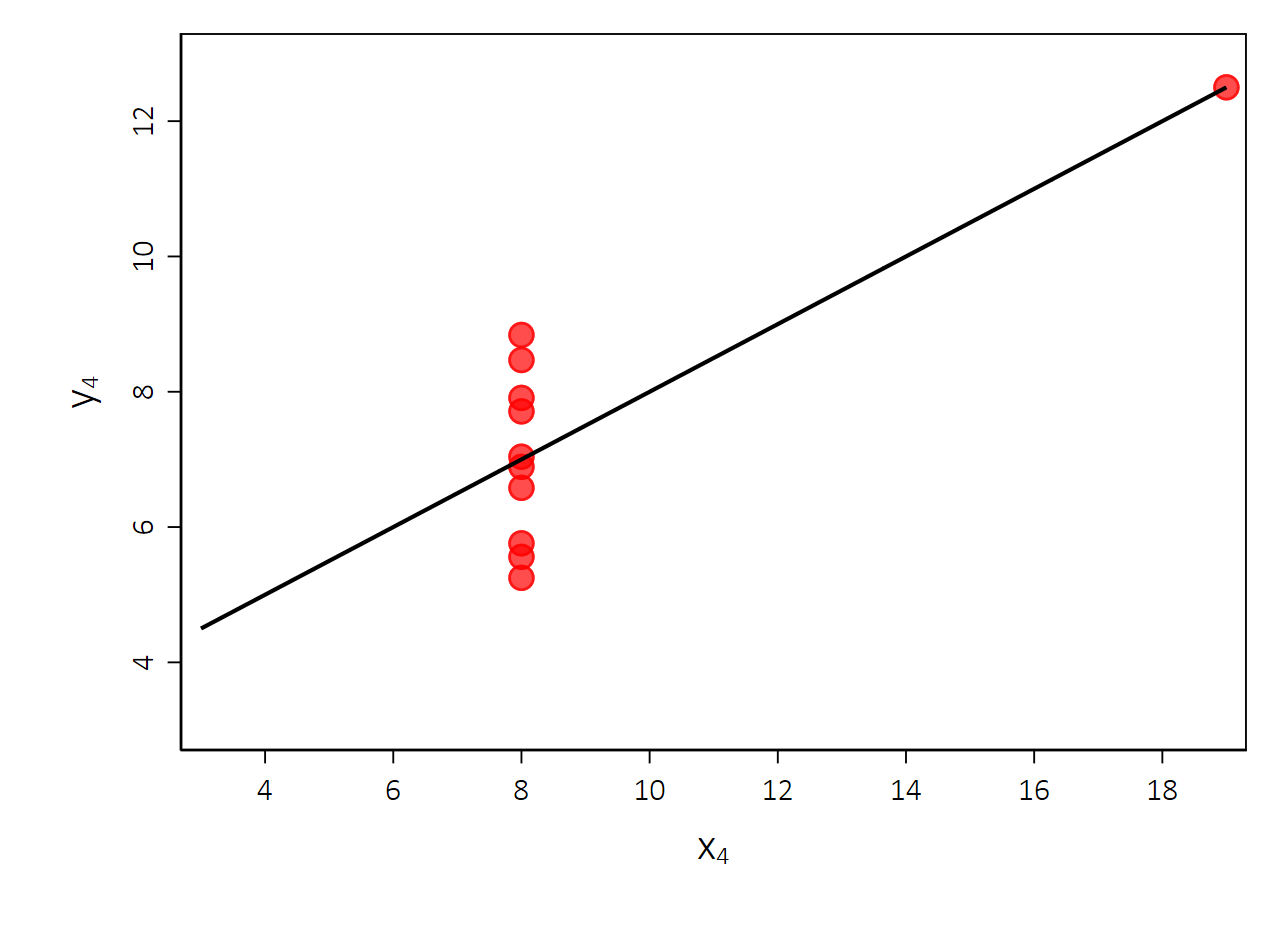
\includegraphics[width=1\textwidth]{figures/Anscombe_data4}
							
  \end{subfigure}
 	\caption{\footnotesize All four sets are identical when examined using linear statistics, but very different when graphed. Correlation between x and y is 0.816. Linear Regression y = 3.00 + 0.50x.}

\end{figure} 
%\end{figure*}
%\end{landscape}
%-------------------------------------------
\end{frame}


\begin{frame}{Data Generating Process: Random Sampling}
%\beamerdefaultoverlayspecification{<+->}

\begin{assumption} \textbf{LRM2: Simple Random Sampling}. 
$$\{x_{i1},\ldots, x_{iK}, y_i\}^N_{i=1} \quad\text{i.i.d. (independent and identically distributed)}$$\pause
\end{assumption}
LRM2 means that
\begin{itemize}
	\item observation $i$ has no information content for observation $j\neq i$\pause
	\item all observations $i$ come from the same distribution\pause
\end{itemize}
This assumption is guaranteed by simple random sampling provided there is no systematic non-response or truncation.

\end{frame}



\begin{frame}{Density of Population and Truncated Sample}
\begin{figure}[t]
	\centering
		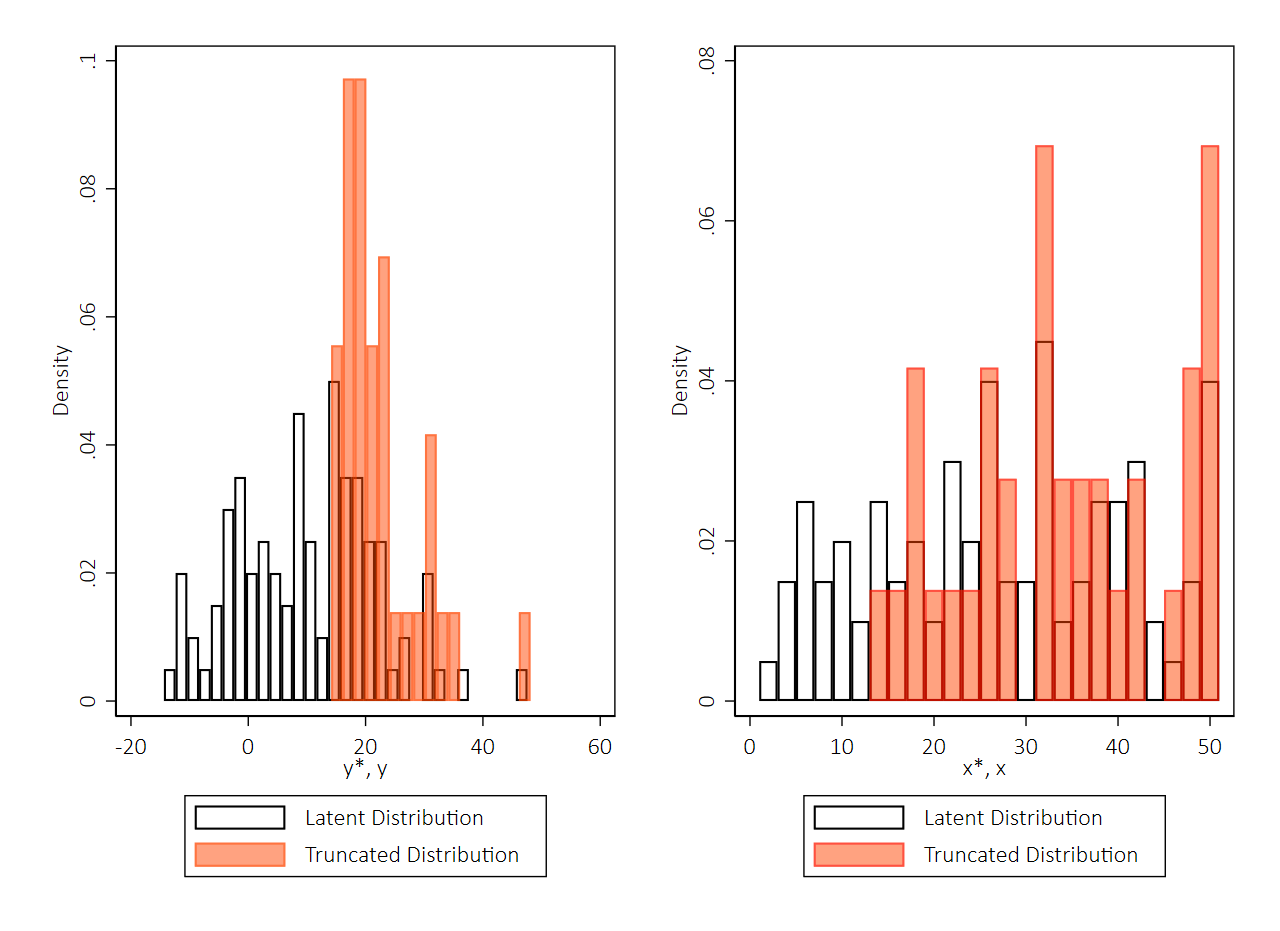
\includegraphics[width=.8\textwidth]{figures/Trunc1}
	\caption{\footnotesize Distribution of a dependent variable and an independent variable truncated at $y^*=15$.\label{fig:LRM}}
\end{figure}
\end{frame}


\begin{frame}{Data Generating Process: Exogeneity}
\scriptsize%\beamerdefaultoverlayspecification{<+->}
\begin{assumption} \textbf{LRM3: Exogeneity}.\pause
\begin{enumerate}[a)]
\item $$u_{i}|x_{i1},\ldots, x_{iK} \sim N(0, \sigma^2_i)$$\pause
LRM3a assumes that the error term is normally distributed conditional on the explanatory variables.\pause
\item $$u_i\; \bot\; x_{ik} \quad \forall k\quad\text{(independent)}, pdf_{u,x}(u_{i}x_{ik})=pdf_{u}(u_{i})pdf_{x}(x_{ik})$$\pause
LRM3b means that the error term is independent of the explanatory variables.\pause
\item $$E(u_{i}|x_{i1},\ldots, x_{iK})=E(u_{i})=0 \quad \text{(mean independent)}$$\pause
LRM3c states that the \emph{mean} of the error term is independent of explanatory variables.\pause
\item $$cov(x_{ik},u_i)=0 \quad \forall k\quad\text{(uncorrelated)}$$\pause
LRM3d means that the error term and the explanatory variables are uncorrelated.\pause
\end{enumerate}\pause
\end{assumption}
LRM3a or LRM3b imply LRM3c and LRM3d. LRM3c implies LRM3d.
\end{frame}


\begin{frame}{(Conditional) Mean Independence}
\begin{figure}[t]
	\centering
		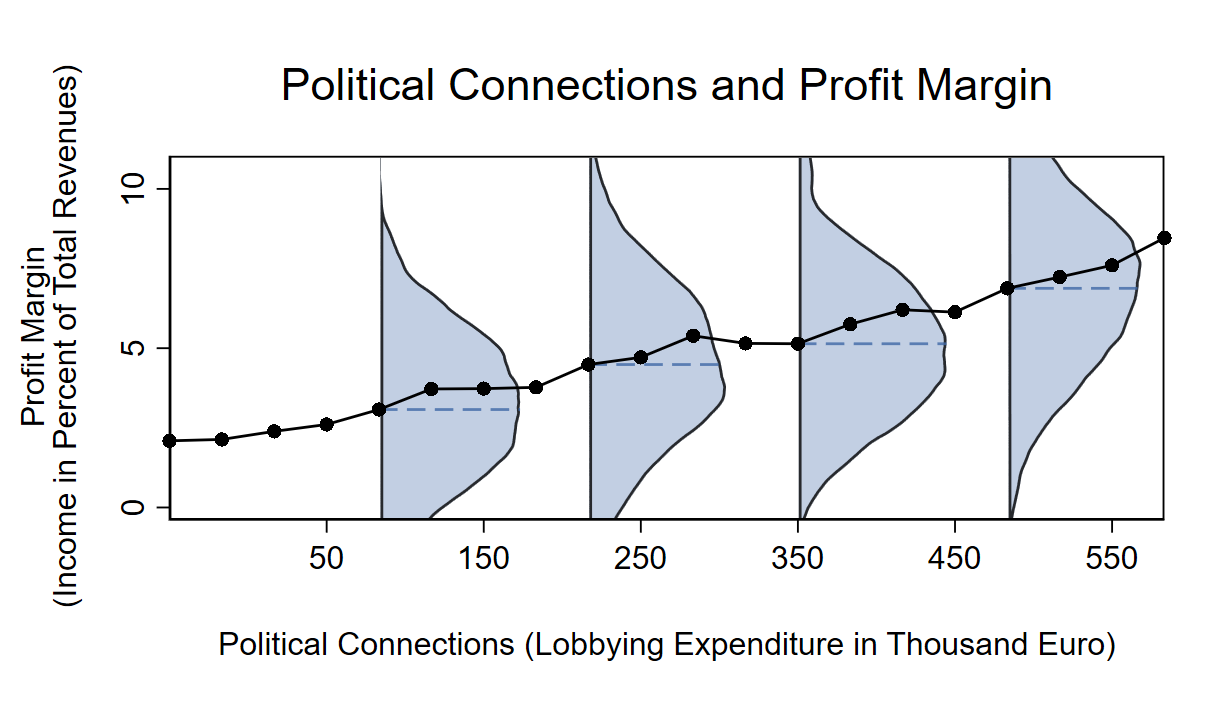
\includegraphics[width=.6\textwidth]{figures/meanindependence_cut}
	\caption{\footnotesize Distributions of the dependent variable conditional on values of an independent variable.\label{fig:LRM}}
\end{figure}
Weaker exogeneity assumption if interest only in, say, $x_{i1}$:\\
\textbf{Conditional Mean Independence} $E(u_{i}|x_{i1},x_{i2},\ldots, x_{iK})=E(u_{i}|x_{i2},\ldots, x_{iK})$\\
Given the control variables $x_{i2},\ldots, x_{iK}$, the mean of $u_i$ does not depend on the variable of interest $x_{i1}$.
\end{frame}


\begin{frame}{Data Generating Process: Error Variance}
%\beamerdefaultoverlayspecification{<+->}
\small \begin{assumption} \textbf{LRM4: Error Variance}.\pause
\begin{enumerate}[a)]
\item $$V(u_{i}|x_{i1},\ldots, x_{iK})=\sigma^2 < \infty \quad \text{(homoskedasticity)}$$\pause
LRM4a means that the variance of the error term is a constant.\pause
\item $$V(u_{i}|x_{i1},\ldots, x_{iK})=\sigma^2_{i} = g(x_{i1},\ldots, x_{iK}) < \infty \quad \text{(cond. heteroskedasticity)}$$\pause
LRM4b allows the variance of the error term to depend on a function $g$ of the explanatory variables.
\end{enumerate}
\end{assumption}
\end{frame}


\begin{frame}{Heteroskedasticity}
\beamerdefaultoverlayspecification{<+->}
\begin{figure}[t]
	\centering
{		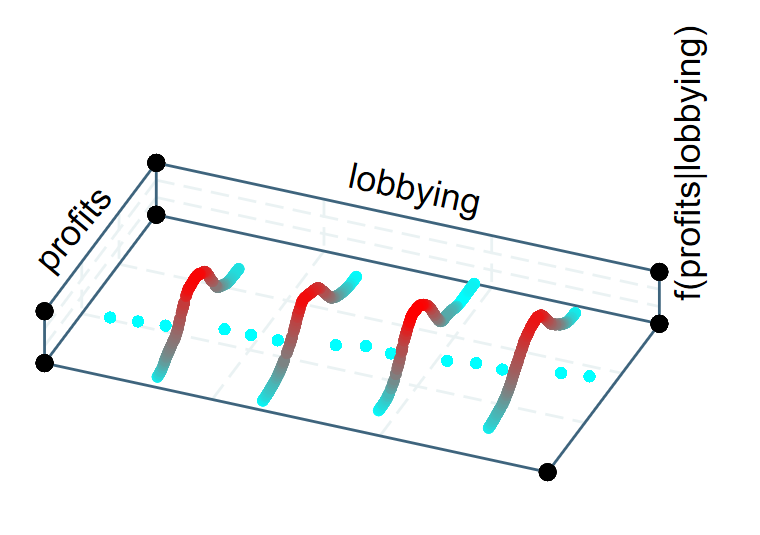
\includegraphics[width=.4\textwidth]{figures/homo.png}}\pause
{		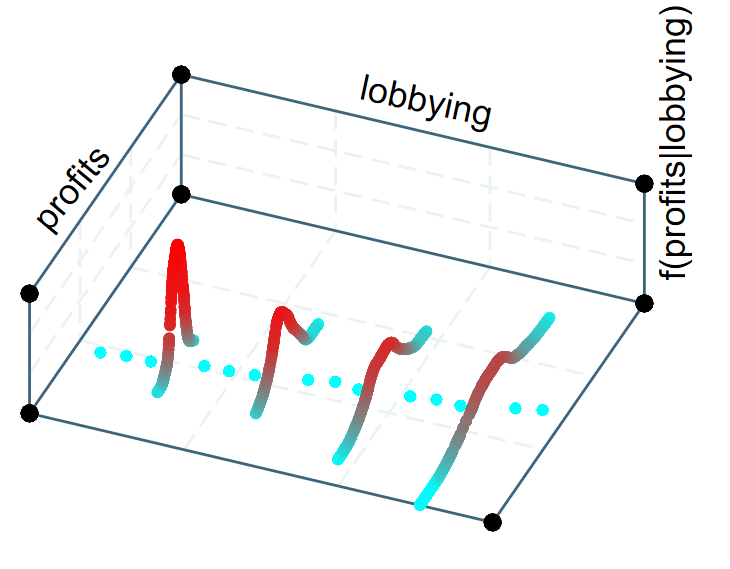
\includegraphics[width=.4\textwidth]{figures/hetero.png}}\pause
	\caption{The simple regression model under homo- and heteroskedasticity. $Var(profits|lobbying, employees)$ increasing with $lobbying$.
	%\cite{Wooldridge2009}.\label{fig:homo}
	}
\end{figure}

\end{frame}


\begin{frame}{Data Generating Process: Identifiability}
%\beamerdefaultoverlayspecification{<+->}
\begin{assumption} \textbf{LRM5: Identifiability}.\pause
$$(x_{i0},x_{i1},\ldots, x_{iK}) \text{ are not linearly dependent}$$\pause
$$0 < V(x_{ik}) < \infty \quad \forall k>0$$\pause
\end{assumption}
LRM5 assumes that \pause
\begin{itemize}
	\item the regressors are not \emph{perfectly collinear}, i.e. no variable is a linear combination of the others\pause
	\item all regressors (but the constant) have strictly positive variance both in expectations and in the sample and not too many extreme values.\pause
\end{itemize}
LRM5 means that every explanatory variable adds additional information.
\end{frame}

\begin{frame}{The Identifying Variation from $x_{ik}$}
\begin{figure}[t]
	\centering
		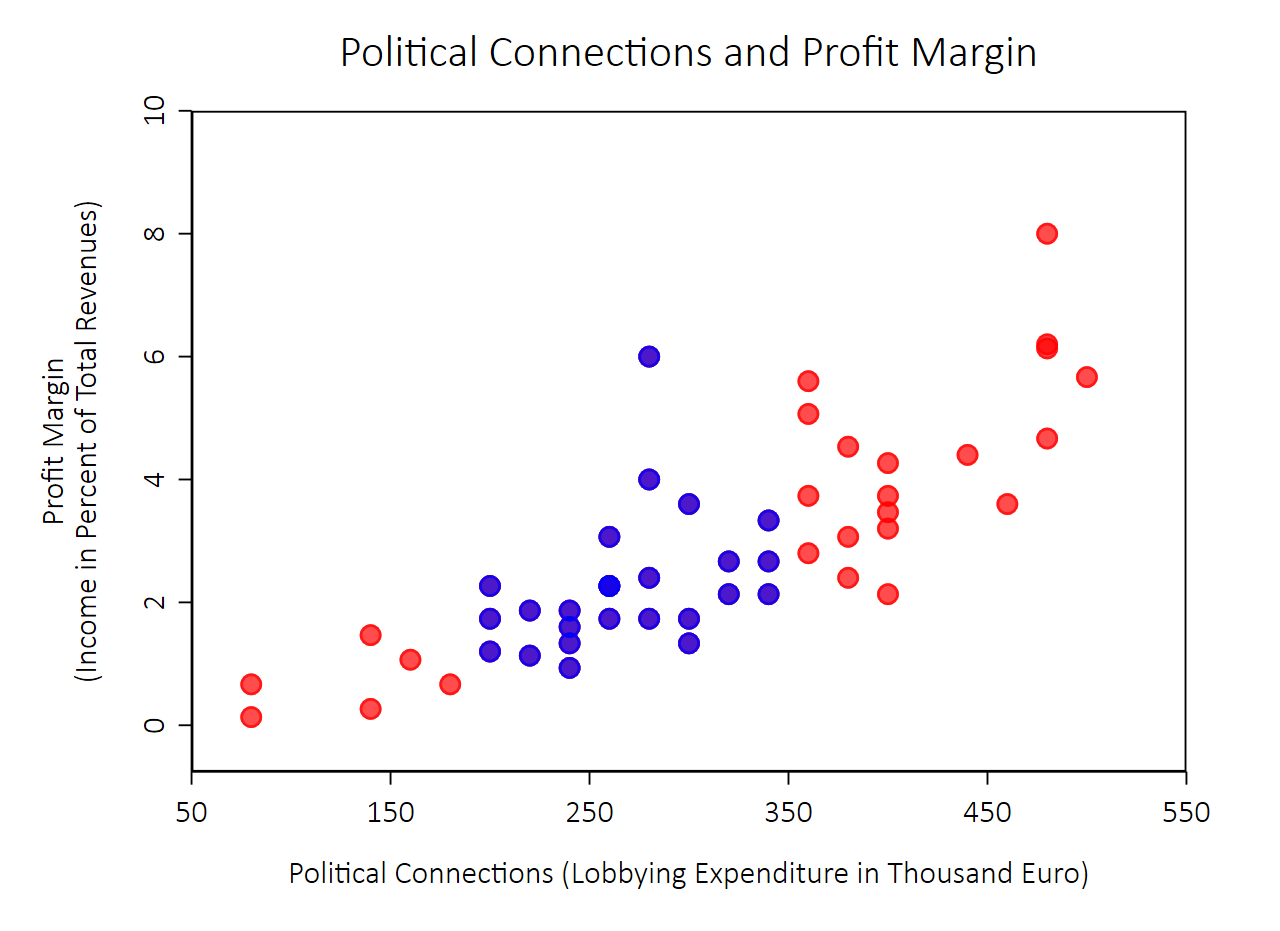
\includegraphics[width=.8\textwidth]{figures/identifiability}
	\caption{The number of red and blue dots is the same. Using which would you get a more accurate regression line? \label{fig:LRM}}
\end{figure}
\end{frame}








\section{Estimation with OLS}

% --------------------------------------------------- Slide --
\begin{frame}
	\frametitle{Content}
	\tableofcontents[%
 		currentsection, % causes all sections but the current to be shown in a semi-transparent way.
 		%currentsubsection, % causes all subsections but the current subsection in the current section to ...
 		%hideallsubsections, % causes all subsections to be hidden.
 		%hideothersubsections, % causes the subsections of sections other than the current one to be hidden.
 		%part=, % part number causes the table of contents of part part number to be shown
 		%pausesections, % causes a \pause command to be issued before each section. This is useful if you
 		%pausesubsections, %  causes a \pause command to be issued before each subsection.
 		%sections={ overlay specification },
	]

\end{frame}


\begin{frame}{Estimation with OLS}
\beamerdefaultoverlayspecification{<+->}
\textbf{Ordinary least squares (OLS)} minimizes the squared distances (SD) between the observed and the predicted dependent variable $y$:\pause
$$\min_{\beta_0,\ldots,\beta_K}{SD(\beta_0,\ldots,\beta_K)},$$\pause
$$\text{where } SD=\sum^{N}_{i=1}{[y_i-(\beta_0+\beta_1x_{i1}+\ldots+\beta_Kx_{iK})]^2}.$$\pause


\end{frame}

\begin{frame}{How to Describe the Relationship Best?}
    \begin{center}
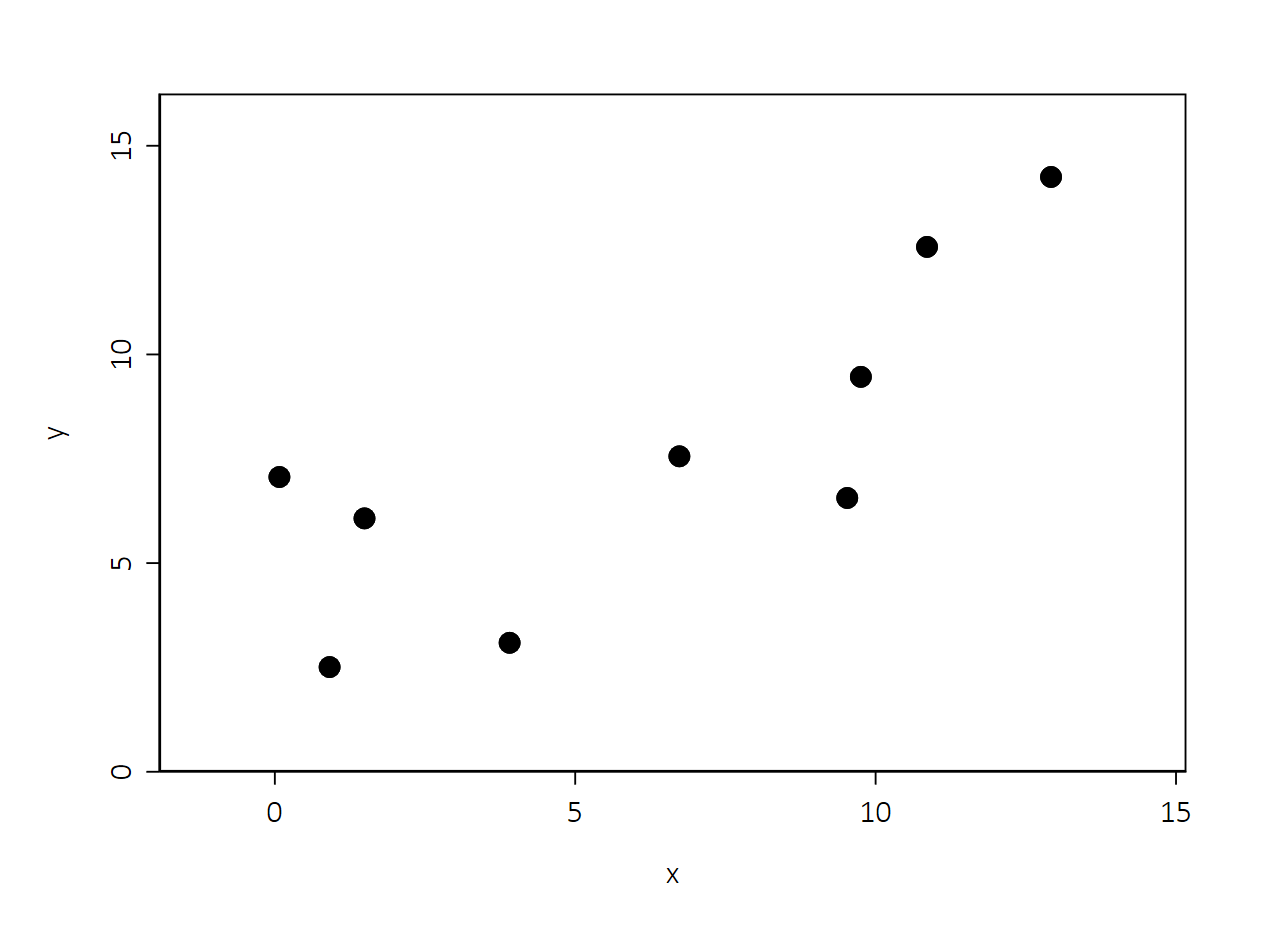
\includegraphics[width=1\textwidth]{figures/OLS1}
     \end{center}
\end{frame}

\begin{frame}{How to Describe the Relationship Best?}
    \begin{center}
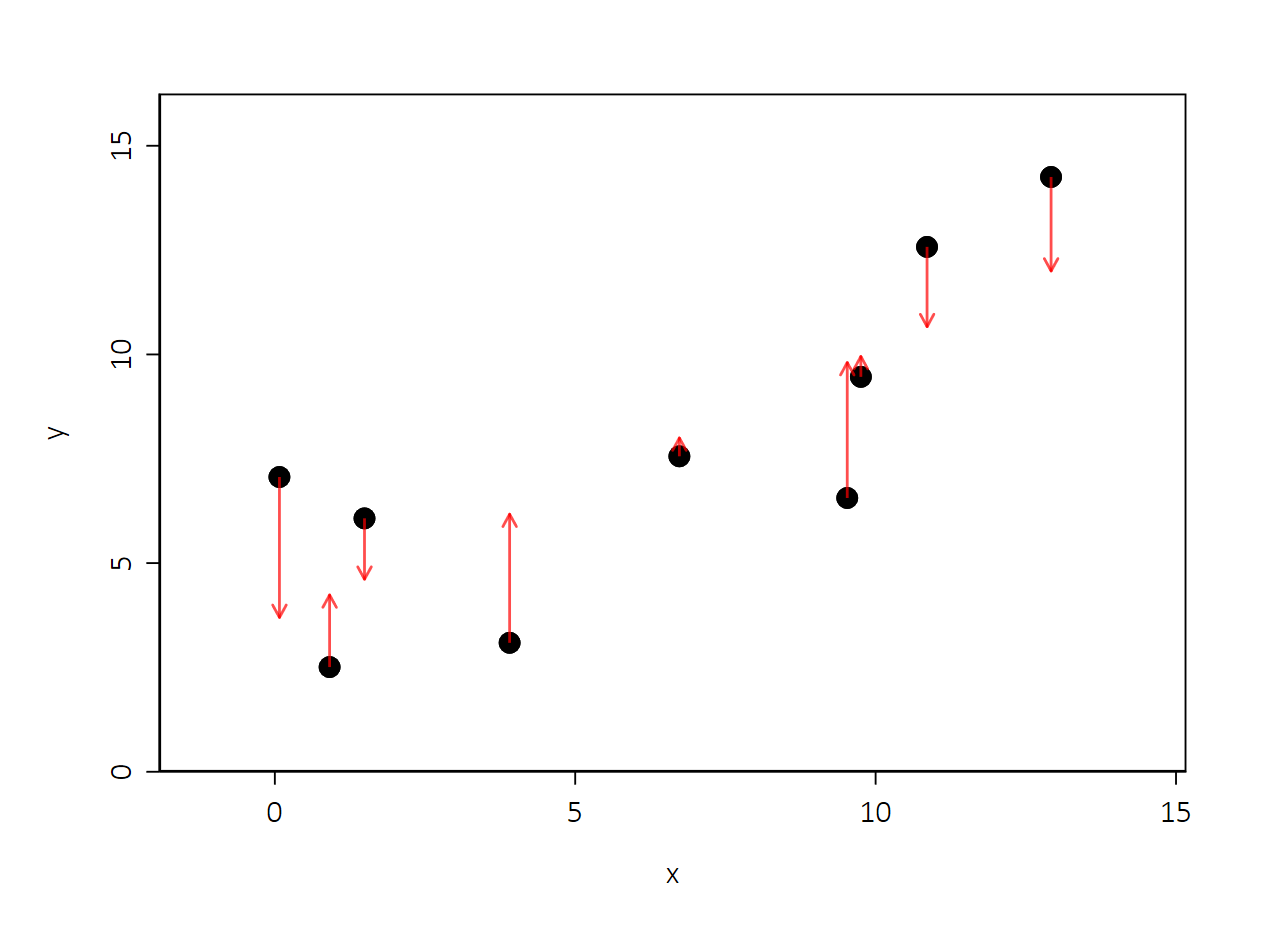
\includegraphics[width=1\textwidth]{figures/OLS2}
     \end{center}
\end{frame}

\begin{frame}{How to Describe the Relationship Best?}
    \begin{center}
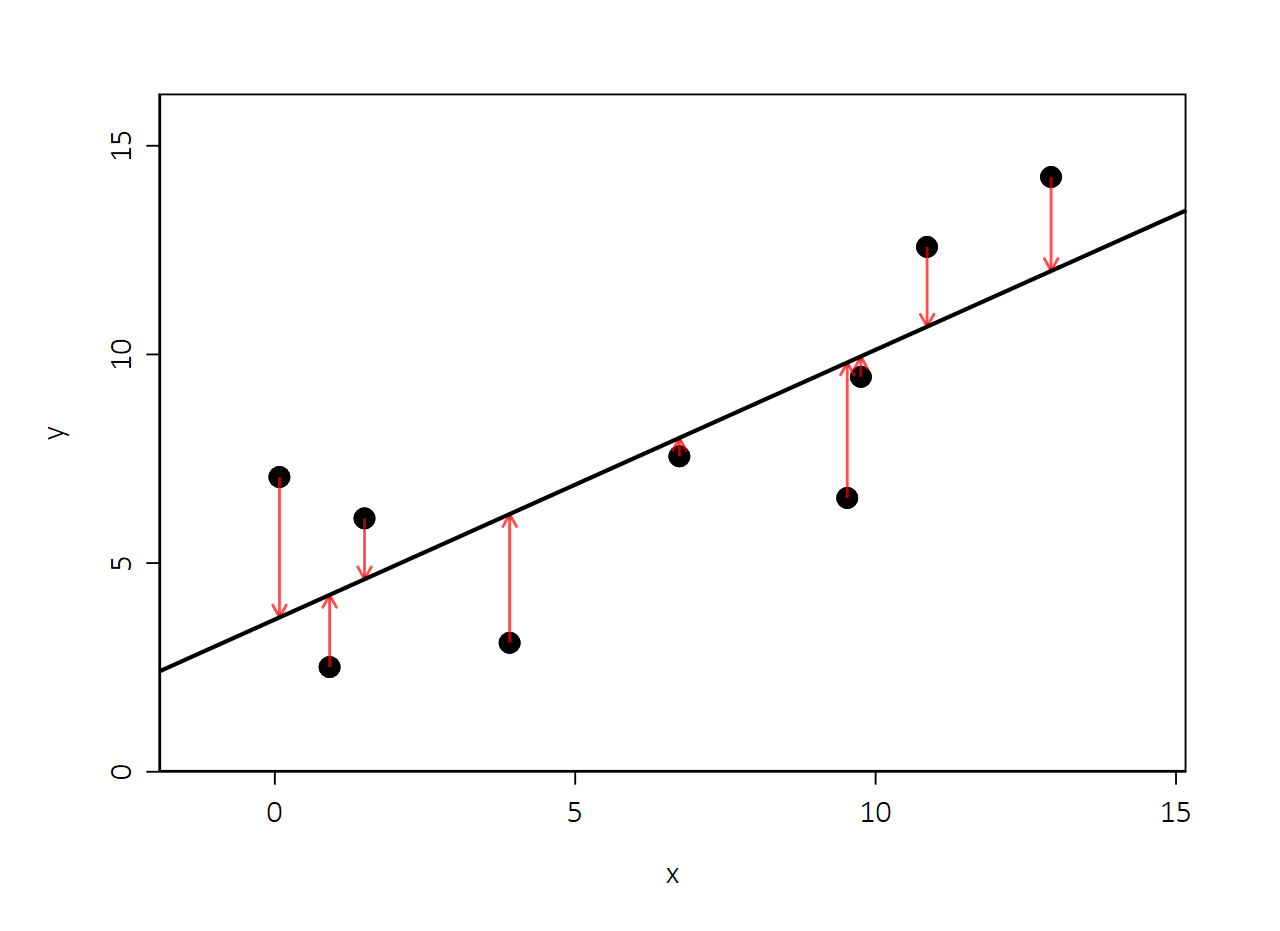
\includegraphics[width=1\textwidth]{figures/OLS3}
     \end{center}
\end{frame}

\begin{frame}{How to Describe the Relationship Best?}
    \begin{center}
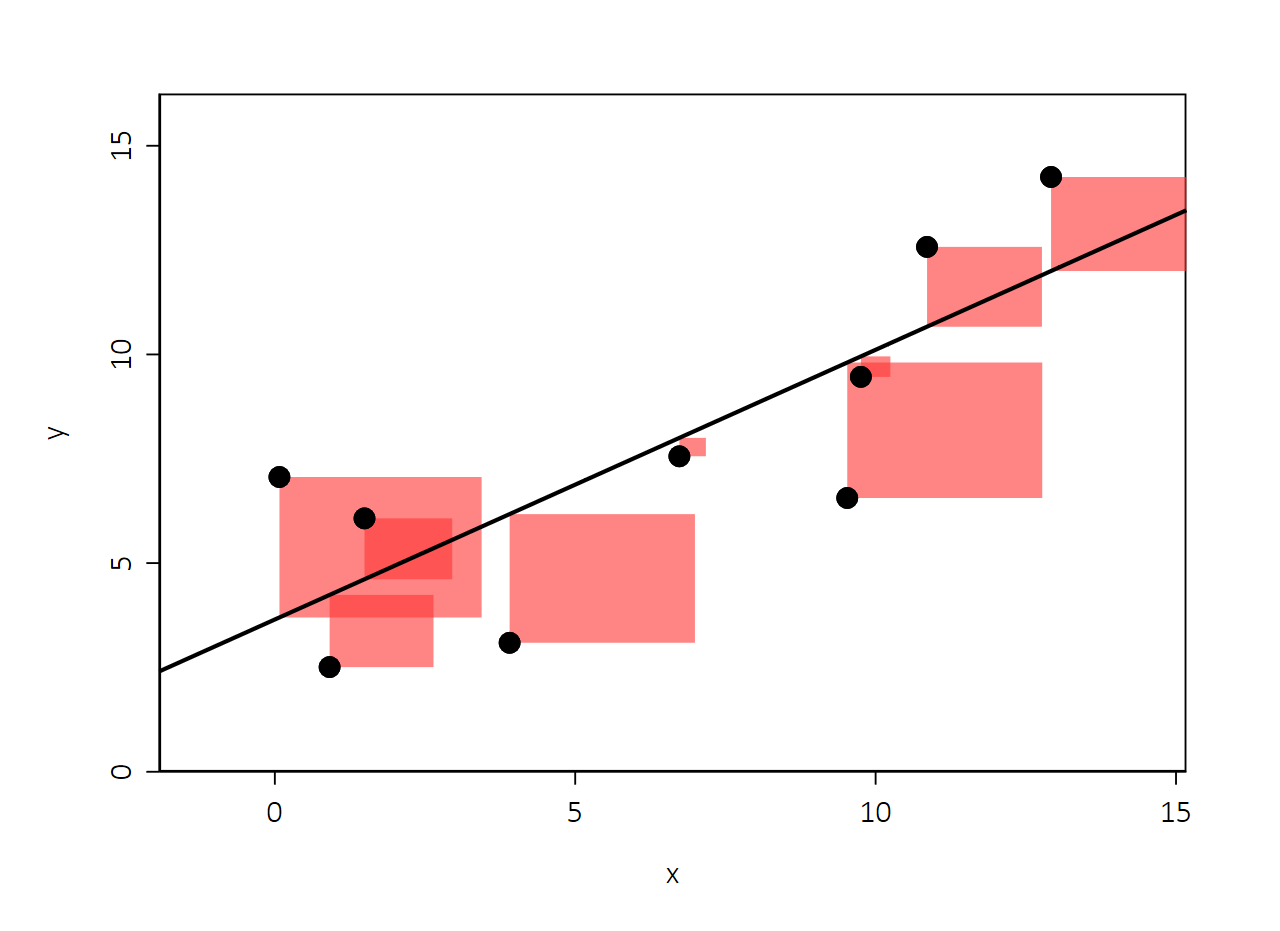
\includegraphics[width=1\textwidth]{figures/OLS4}
     \end{center}
\end{frame}


\begin{frame}{How to Describe the Relationship Best?}
    \begin{center}
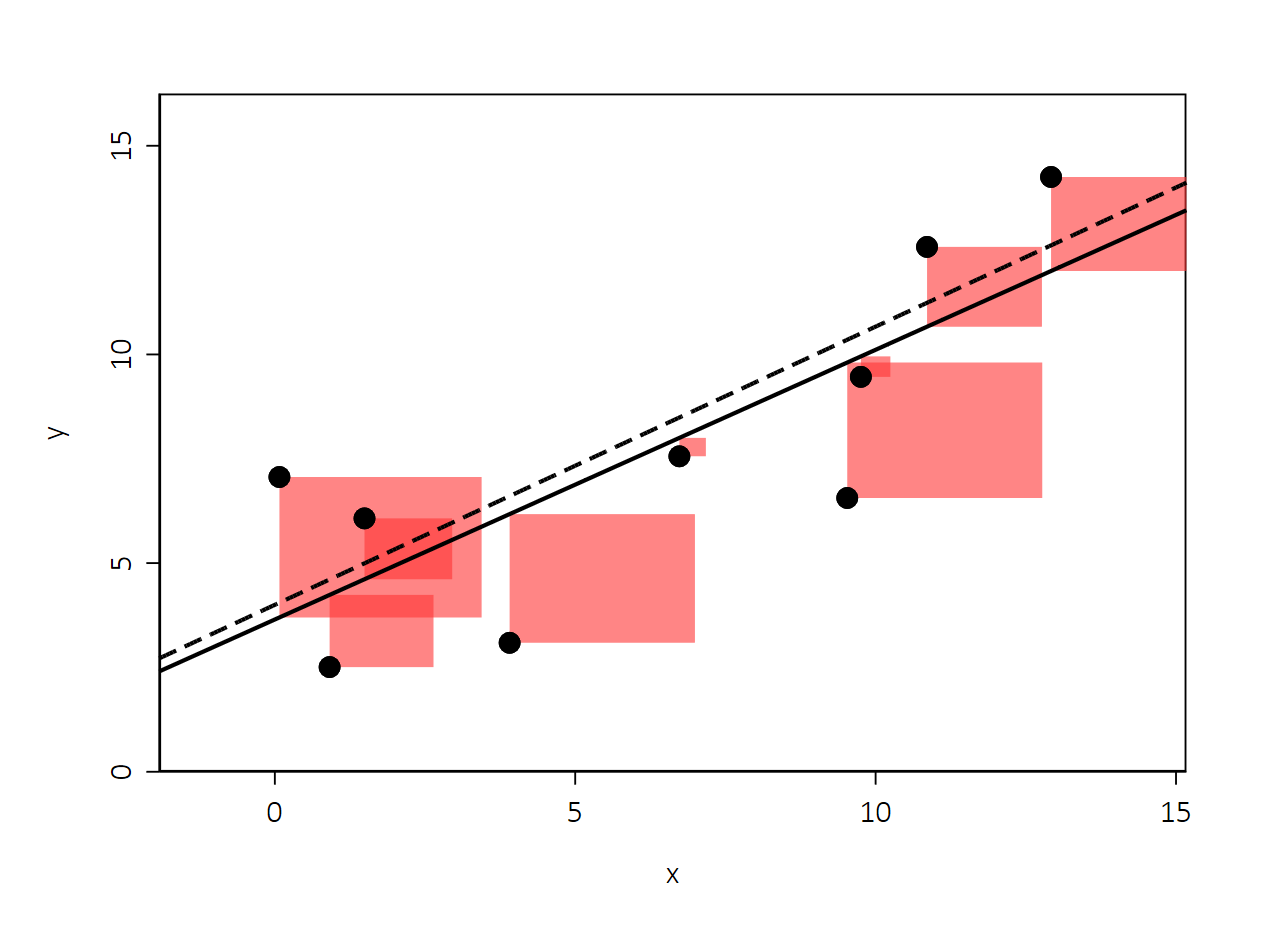
\includegraphics[width=1\textwidth]{figures/OLS5}
     \end{center}
\end{frame}




\begin{frame}{Invention of OLS}
%\beamerdefaultoverlayspecification{<+->}

\begin{columns}
\begin{column}{0.45\textwidth}
\small
Legendre to Jacobi (Paris, 30 November 1827, \citealp{Plackett1972}): ``\textit{...How can Mr. Gauss have dared to tell you that the greater part of your theorems were known to him...?}\\[1ex]\pause \textit{ ... this is the same man ... who wanted to appropriate in 1809 the method of least squares published in 1805.}\\[2ex]\pause \textit{--- Other examples will be found in other places, but a man of honour should refrain from imitating them.}''\pause


\end{column}
\begin{column}{0.55\textwidth}  %%<--- here
\begin{figure}[t]
	\centering
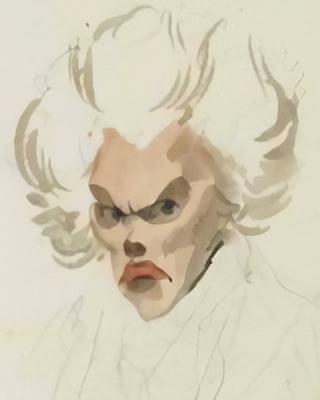
\includegraphics[width=0.55\textwidth]{figures/Legendre}
	\caption{\footnotesize Watercolor caricature of Legendre by Boilly (1820), the only existing portrait known.}
\end{figure}
\end{column}
\end{columns}

\end{frame}


\begin{frame}{Invention of OLS}
%\beamerdefaultoverlayspecification{<+->}

\begin{columns}
\begin{column}{0.45\textwidth}
\small
Legendre to Jacobi (Paris, 30 November 1827, \citealp{Plackett1972}): ``\textit{...How can Mr. Gauss have dared to tell you that the greater part of your theorems were known to him...?}\\[1ex] \textit{ ... this is the same man ... who wanted to appropriate in 1809 the method of least squares published in 1805.}\\[2ex] \textit{--- Other examples will be found in other places, but a man of honour should refrain from imitating them.}''


\end{column}
\begin{column}{0.55\textwidth}  %%<--- here
\begin{figure}[t]
	\centering
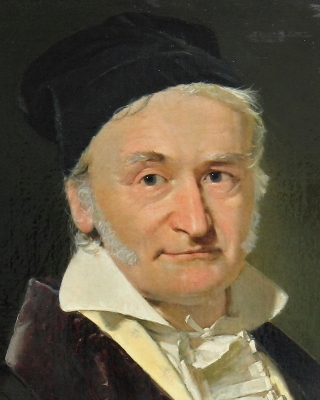
\includegraphics[width=0.55\textwidth]{figures/Gauss_klein}
	\caption{\footnotesize Portrait of Gauss by Jensen (1840).}
\end{figure}
\end{column}
\end{columns}

\end{frame}

\begin{frame}{Estimation with OLS}
\beamerdefaultoverlayspecification{<+->}
For the bivariate regression model, the OLS estimators of $\beta_0$ and $\beta_1$ are \pause\\

$$\hat{\beta}_0=\bar{y}-\hat{\beta}_1\bar{x}$$\pause
$$\hat{\beta}_1=\frac{\sum^{N}_{i=1}{(x_{i1}-\bar{x})(y_{i}-\bar{y})}}{\sum^{N}_{i=1}{(x_{i1}-\bar{x})^2}}=\frac{cov(x,y)}{var(x)}$$\pause


$$\hat{\beta}_1=cov(x,y)/(s_xs_x)=Rs_y/s_x,$$
where $R\equiv cov(x,y)/(s_xs_y)$ is \textbf{Pearson's correlation coefficient} with $s_z$ denoting the standard deviation of $z$.

%That is, the slope coefficient is equal to the correlation coefficient $R$ times the ratio of standard deviations of $y$ and $x$.


\end{frame}

\begin{frame}{OLS estimator Measures Linear Correlation}
\beamerdefaultoverlayspecification{<+->}
Equivalently,
$$R=s_x/s_y \hat{\beta}_1= \frac{\hat{\beta}_1\sum^{N}_{i=1}{(x_{i1}-\bar{x}})}{\sum^{N}_{i=1}{(y_{i}-\bar{y})}}=\frac{\sum^{N}_{i=1}{(\hat{\beta}_1x_{i1}-\hat{\beta}_1\bar{x}})}{\sum^{N}_{i=1}{(y_{i}-\bar{y})}}.$$

Squaring gives
$$R^2 =\frac{\sum^{N}_{i=1}{(\hat{y}_{i}-\bar{y})^2}}{\sum^{N}_{i=1}{(y_{i}-\bar{y})^2}}=1 - \frac{\sum^{N}_{i=1}{\hat{u}^2_{i}}}{\sum^{N}_{i=1}{(y_{i}-\bar{y})^2}}.$$
$R^2$ as measure of the \textbf{goodness of fit}:\\The fit improves with the fraction of the sample variation in $y$ that is explained by the $x$.
\end{frame}


\begin{frame}{The Case with $K$ Explanatory Variables}
\beamerdefaultoverlayspecification{<+->}


\begin{columns}
\begin{column}{0.45\textwidth}
\small
The more general case with $K$ explanatory variables is 
$$\underset{(K+1) \times 1}{\hat{\beta}}=\underset{(K+1) \times (K+1)}{(X'X)^{-1}}\;\underset{(K+1) \times N}{X'}\;\underset{N \times 1}{y}$$\pause

\end{column}
\begin{column}{0.55\textwidth}  %%<--- here
		\begin{figure}[t]
	\centering
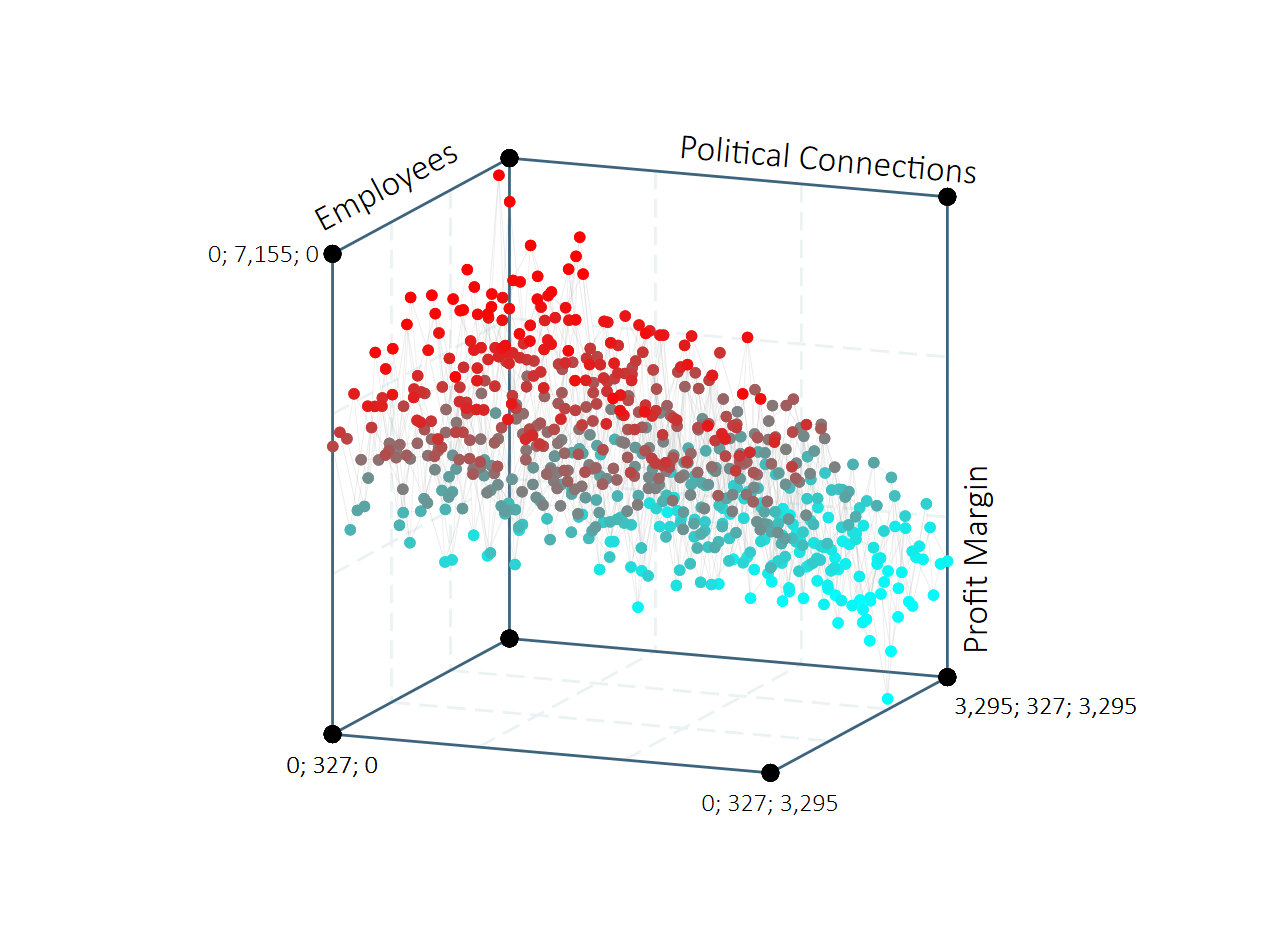
\includegraphics[width=0.8\textwidth]{figures/3d_cloud1}
	\caption{\scriptsize Scatter cloud visualized with\\ \textcolor{persianred}{GRAPH3D for Stata}.\label{fig:LRM}}
\end{figure}
\end{column}
\end{columns}
\pause

Given the OLS estimator, we can predict the
\begin{itemize}
	\item dependent variable by $\hat{y_i} = \hat{\beta}_0 + \hat{\beta}_1x_{i1} + \ldots + \hat{\beta}_K x_{iK}$\pause
	\item the error term by $\hat{u}_i = y_i - \hat{y}_i$.\pause
\end{itemize}
  $\hat{u}_i$ is called the \emph{residual}.\\[2ex]\pause

\textbf{Adjusted $R^2$} $= 1 - \frac{N-1}{N-K-1}\frac{\sum^{N}_{i=1}{\hat{u}^2_{i}}}{\sum^{N}_{i=1}{(y_{i}-\bar{y})^2}}.$

\end{frame}

\begin{frame}{The Case with $K$ Explanatory Variables}
%\beamerdefaultoverlayspecification{<+->}


\begin{columns}
\begin{column}{0.45\textwidth}
\small
The more general case with $K$ explanatory variables is 
$$\underset{(K+1) \times 1}{\hat{\beta}}=\underset{(K+1) \times (K+1)}{(X'X)^{-1}}\;\underset{(K+1) \times N}{X'}\;\underset{N \times 1}{y}$$

\end{column}
\begin{column}{0.55\textwidth}  %%<--- here
		\begin{figure}[t]
	\centering
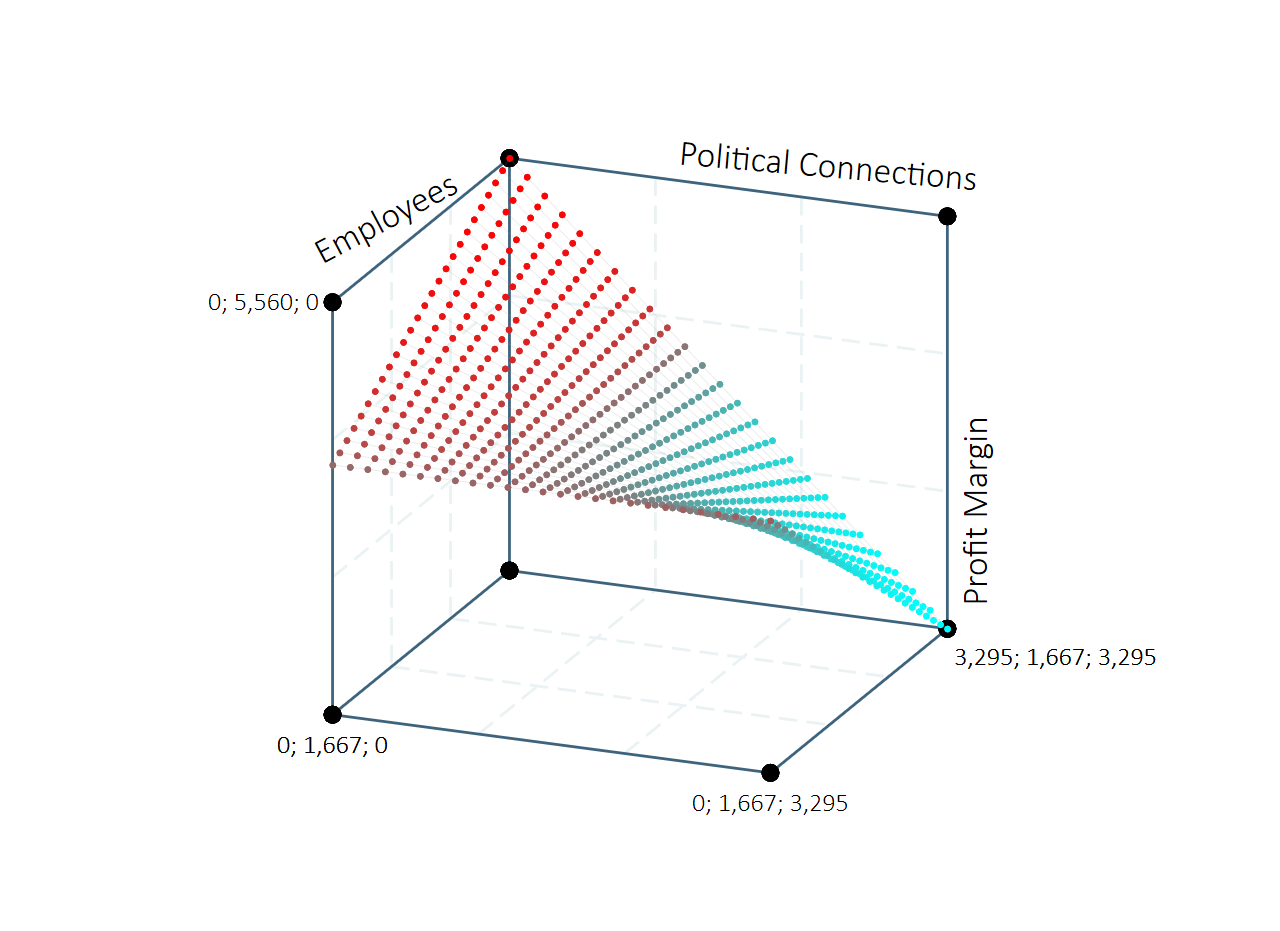
\includegraphics[width=0.8\textwidth]{figures/3d_cloud2}
	\caption{\scriptsize OLS surface visualized with\\ \textcolor{persianred}{GRAPH3D for Stata}.\label{fig:LRM}}
\end{figure}
\end{column}
\end{columns}


Given the OLS estimator, we can predict the
\begin{itemize}
	\item dependent variable by $\hat{y_i} = \hat{\beta}_0 + \hat{\beta}_1x_{i1} + \ldots + \hat{\beta}_K x_{iK}$
	\item the error term by $\hat{u}_i = y_i - \hat{y}_i$.
\end{itemize}
  $\hat{u}_i$ is called the \emph{residual}.\\[2ex]

\textbf{Adjusted $R^2$} $= 1 - \frac{N-1}{N-K-1}\frac{\sum^{N}_{i=1}{\hat{u}^2_{i}}}{\sum^{N}_{i=1}{(y_{i}-\bar{y})^2}}.$

\end{frame}


\section{Properties of the OLS Estimator in the Small and in the Large}

 %--------------------------------------------------- Slide --
\begin{frame}
	\frametitle{Content}
	\tableofcontents[%
 		currentsection, % causes all sections but the current to be shown in a semi-transparent way.
 		%currentsubsection, % causes all subsections but the current subsection in the current section to ...
 		%hideallsubsections, % causes all subsections to be hidden.
 		%hideothersubsections, % causes the subsections of sections other than the current one to be hidden.
 		%part=, % part number causes the table of contents of part part number to be shown
 		%pausesections, % causes a \pause command to be issued before each section. This is useful if you
 		%pausesubsections, %  causes a \pause command to be issued before each subsection.
 		%sections={ overlay specification },
	]

\end{frame}


\begin{frame}{Properties of the OLS Estimator}
\beamerdefaultoverlayspecification{<+->}


\begin{itemize}
	\item \emph{Small sample properties of $\hat{\beta}$}
\begin{itemize}
	\item unbiased
	\item normally distributed
	\item efficient\\[4ex]
\end{itemize}
	\item \emph{Large sample properties of $\hat{\beta}$}
\begin{itemize}
	\item consistent
	\item approx. normal
	\item asymptotically efficient
\end{itemize}
\end{itemize}


\end{frame}


\begin{frame}{Small Sample Properties}
\begin{figure}[t]
	\centering
		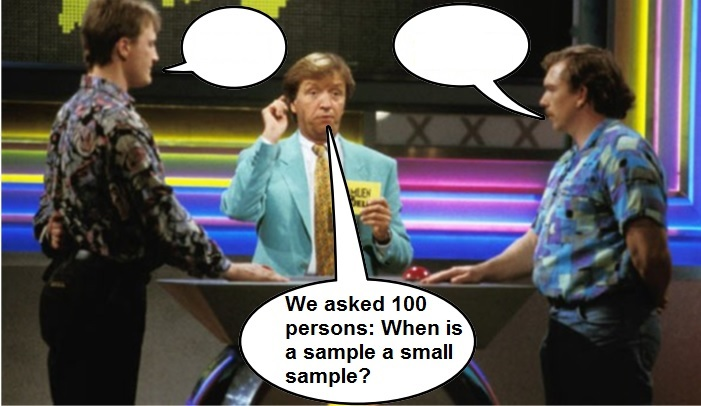
\includegraphics[width=.9\textwidth]{figures/SmallSample_empty.jpg}
	\caption{What is a small sample?\hspace{\textwidth} \emph{Source:} Familien-Duell \hspace{\textwidth}Grundy Light Entertainment. \label{fig:SS}}
\end{figure}
\end{frame}


\begin{frame}{Small Sample Properties}
\begin{figure}[t]
	\centering
		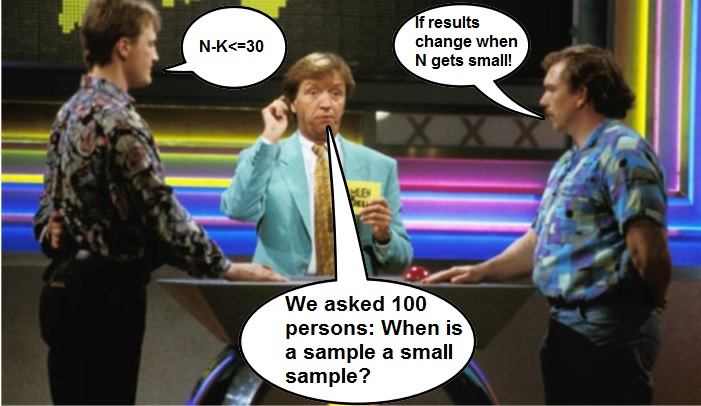
\includegraphics[width=.9\textwidth]{figures/SmallSample.jpg}
	\caption{What is a small sample? \cite[p. 755]{Wooldridge2009}: ``But large sample approximations have been known to work well for sample sizes as small as $N = 20$.''  \emph{Source:} Familien-Duell Grundy Light Entertainment. \label{fig:SS}}
\end{figure}
\end{frame}

\begin{frame}{Unbiasedness and Normality of $\hat{\beta}_k$}
\beamerdefaultoverlayspecification{<+->}
Assuming LRM1, \pause LRM2, \pause LRM3a, \pause LRM4, and \pause LRM5,\\ \pause the following properties can be established even for small samples.\pause
\beX
\item The OLS estimator of $\beta$ is \textbf{unbiased}.\\\pause
$$E(\hat{\beta}_k|x_{11},\ldots,x_{NK})=\beta_k.$$\pause

\item The OLS estimator is (multivariate) \textbf{normally distributed}.\\\pause
$$\hat{\beta}_k|x_{11},\ldots,x_{NK}\sim N(\beta_k,V(\hat{\beta}_k)).$$\pause

\item Under homoskedasticity (LRM4a)\\ the variance $\widehat{V}(\hat{\beta}_k|x_{11},\ldots,x_{NK})$ can be \textbf{unbiasedly} estimated.
\eeX
\end{frame}

\begin{frame}{Variance of $\hat{\beta}_k$ and Efficiency}
\beamerdefaultoverlayspecification{<+->}
\beX
\item For the bivariate regression model, it is estimated as\pause
$$\widehat{V}=\frac{\hat{\sigma}^2}{\sum^{N}_{i=1}{(x_i-\bar{x})^2}} \text{ with}$$\pause
$$\hat{\sigma}^2=\frac{\sum^{N}_{i=1}{\hat{u}^2_i}}{N-K-1}.$$\pause
\item Gau{\ss}-Markov-Theorem: under homoskedasticity (LRM4a)\\$\hat{\beta}_k$ is the \textbf{BLUE} (best linear unbiased estimator, e.g., non-linear least squares biased).
\item $\widehat{V}(\hat{\beta}_k)$ inflates with
\begin{itemize}
	\item \textbf{micronumerosity} (small sample size)
	\item \textbf{multicollinearity} (high (but not perfect) correlation between two or more of the independent variables).
\end{itemize}
\eeX
\end{frame}


\begin{frame}{Unbiasedness}
\beamerdefaultoverlayspecification{<+->}
\beX
\item The OLS estimator of $\beta$ is \emph{unbiased}.\\
Plug $y=X\beta+u$ into the formula for $\hat\beta$ and then use the law of iterated expectation to first take expectation with respect to $u$ conditional
on $X$ and then take the unconditional expectation:\pause

$$\operatorname{E}[\,\hat\beta] = E_{X,u}\Big[(X'X)^{-1}X'(X\beta+u)\Big]$$ \pause
$$= \beta + E_{X,u}\Big[(X'X)^{-1}X'u\Big]$$ \pause
$$= \beta + E_{X}\Big[E_{u|X}\Big[(X'X)^{-1}X'u|X \Big]\Big] $$\pause
$$= \beta + E_{X}\Big[(X'X)^{-1}X'E_{u|X}[u|X]\Big]$$\pause
$$= \beta,$$\\\pause

where $E[u|X]=0$ by assumptions of the model.\qed
\eeX
\end{frame}


\begin{frame}{Variance}
\beamerdefaultoverlayspecification{<+->}
\beX
\item The OLS estimator $\beta$ has variance $\widehat{V}(\hat{\beta}_k|x_{11},\ldots,x_{NK}) = \sigma^2 (X'X)^{-1}$ \\\pause
Let $\sigma^2 I$ denote the covariance matrix of $u$. Then,  

$$E[\,(\hat\beta - \beta)(\hat\beta - \beta)'] = E\Big[ ((X'X)^{-1}X'u)((X'X)^{-1}X'u)' \Big] $$\pause
$$= E\Big[ (X'X)^{-1}X'uu'X(X'X)^{-1} \Big] $$\pause
$$= E\Big[ (X'X)^{-1}X'\sigma^2X(X'X)^{-1} \Big] $$\pause
$$= E\Big[ \sigma^2(X'X)^{-1}X'X(X'X)^{-1} \Big] $$\pause
$$= \sigma^2 (X'X)^{-1}, $$

where we used the fact that $\hat{\beta} - \beta $ is just an affine transformation of $u$ by the matrix $(X'X)^{-1}X'$. 
\qed

\eeX
\end{frame}

\begin{frame}{Estimator for Variance}
\beamerdefaultoverlayspecification{<+->}
\scriptsize
For a simple linear regression model, where $\beta = [\beta_0,\beta_1]'$ ($\beta_0$ is the y-intercept and $\beta_1$ is the slope), one obtains

$$\sigma^2 (X'X)^{-1} =  \sigma^2 \left(\sum x_ix_i'\right)^{-1}$$\pause
$$=  \sigma^2 \left(\sum (1,x_i)' (1,x_i) \right)^{-1}$$\pause
$$=  \sigma^2 \left(\sum \begin{pmatrix} 1 x_i\\x_i x_i^2\end{pmatrix} \right)^{-1}$$\pause
$$=  \sigma^2 \begin{pmatrix} N \sum x_i\\\sum x_i \sum x_i^2\end{pmatrix}^{-1}$$\pause
$$=  \sigma^2 \cdot \frac{1}{N\sum x_i^2-(\sum x_i)^2}\begin{pmatrix} \sum x_i^2 -\sum x_i\\-\sum x_i N\end{pmatrix}$$\pause
$$=  \sigma^2 \cdot \frac{1}{N\sum_{i=1}^N{(x_i - \bar{x})^2}}\begin{pmatrix} \sum x_i^2 -\sum x_i\\-\sum x_i N\end{pmatrix}$$\pause
$$Var(\beta_1) = \frac{\sigma^2}{\sum_{i=1}^N{(x_i - \bar{x})^2}}.$$

\end{frame}


\begin{frame}{Parameter Values for Simulations}
\beamerdefaultoverlayspecification{<+->}


\textbf{Monte Carlo Simulations} show the distribution of the estimate.
Suppose the data generating process is
$$y_i = \beta_0 + \beta_1 x_{i1} + u_{i}.$$
\begin{columns}
\begin{column}{0.45\textwidth}
\small
\begin{itemize}
	\item $\beta_0 = 2.00$
	\item $\beta_1 =0.5$
	\item $u_i\sim N(0.00,1.00)$
	\item $N=3, N=5, N=10,$\\$N=25, N=100, N=1000$
\end{itemize}
\end{column}
\begin{column}{0.55\textwidth}  %%<--- here
Try it yourself...
\end{column}
\end{columns}

\end{frame}
\begin{frame}{How to Establish Asymptotic Properties of $\hat{\beta}_k$?}
%\beamerdefaultoverlayspecification{<+->}
\begin{columns}
\begin{column}{0.45\textwidth}
\small\pause
\textbf{Law of Large Numbers}\\\pause
As $N$ increases, the distribution of $\hat{\beta}_k$ becomes more tightly centered around $\beta_k$.\pause
\end{column}
\begin{column}{0.55\textwidth}  %%<--- here
%-------------------------------------------
\begin{figure}[htbp]
	\begin{subfigure}[c]{0.49\textwidth}
		\centering
		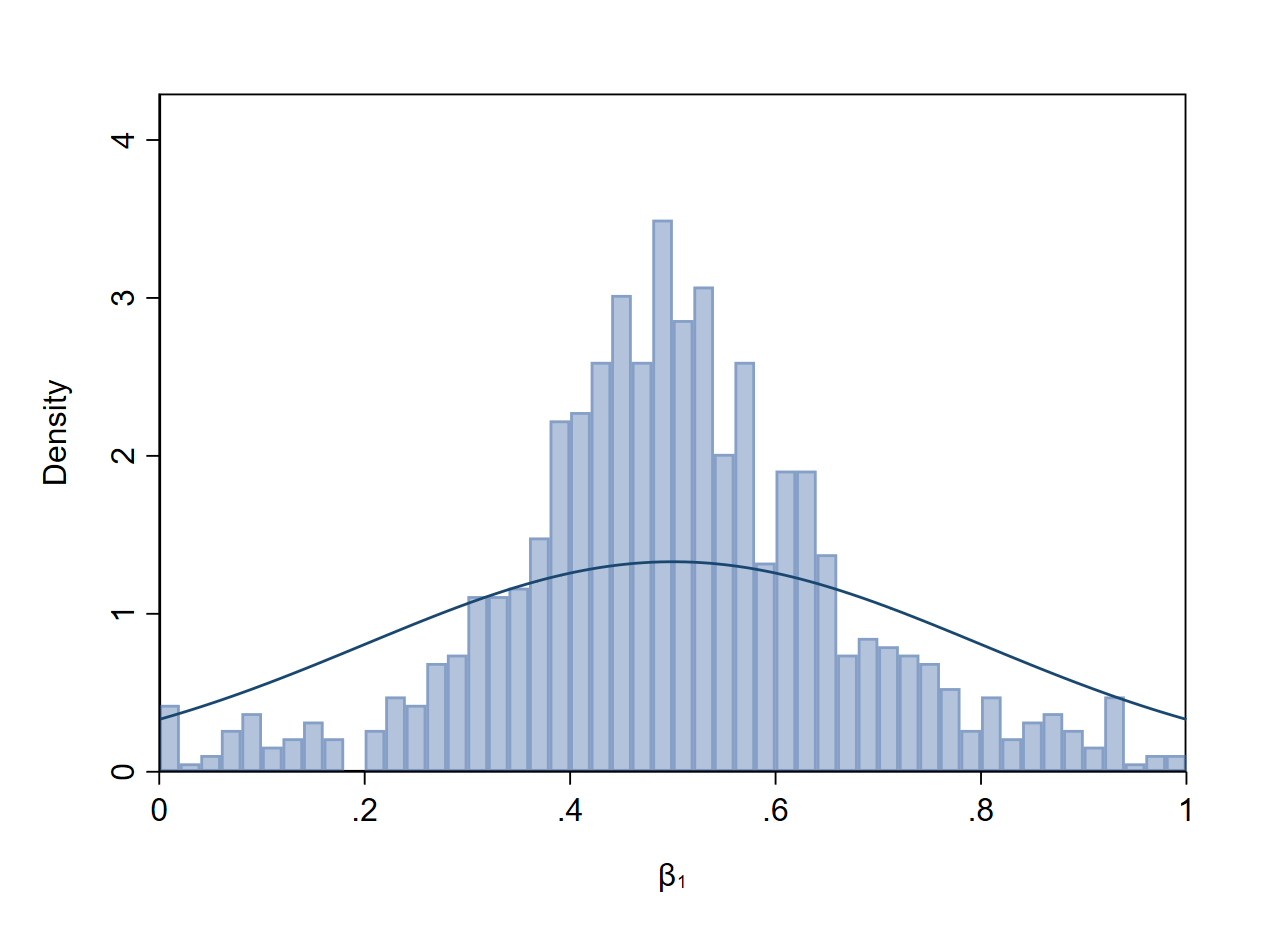
\includegraphics[width=1\textwidth]{figures/distribution_beta1_3}
		\caption{N=3}
    \label{fig:distribution beta1 N3}
	\end{subfigure}%
	\pause
	\begin{subfigure}[c]{0.49\textwidth}
		\centering
		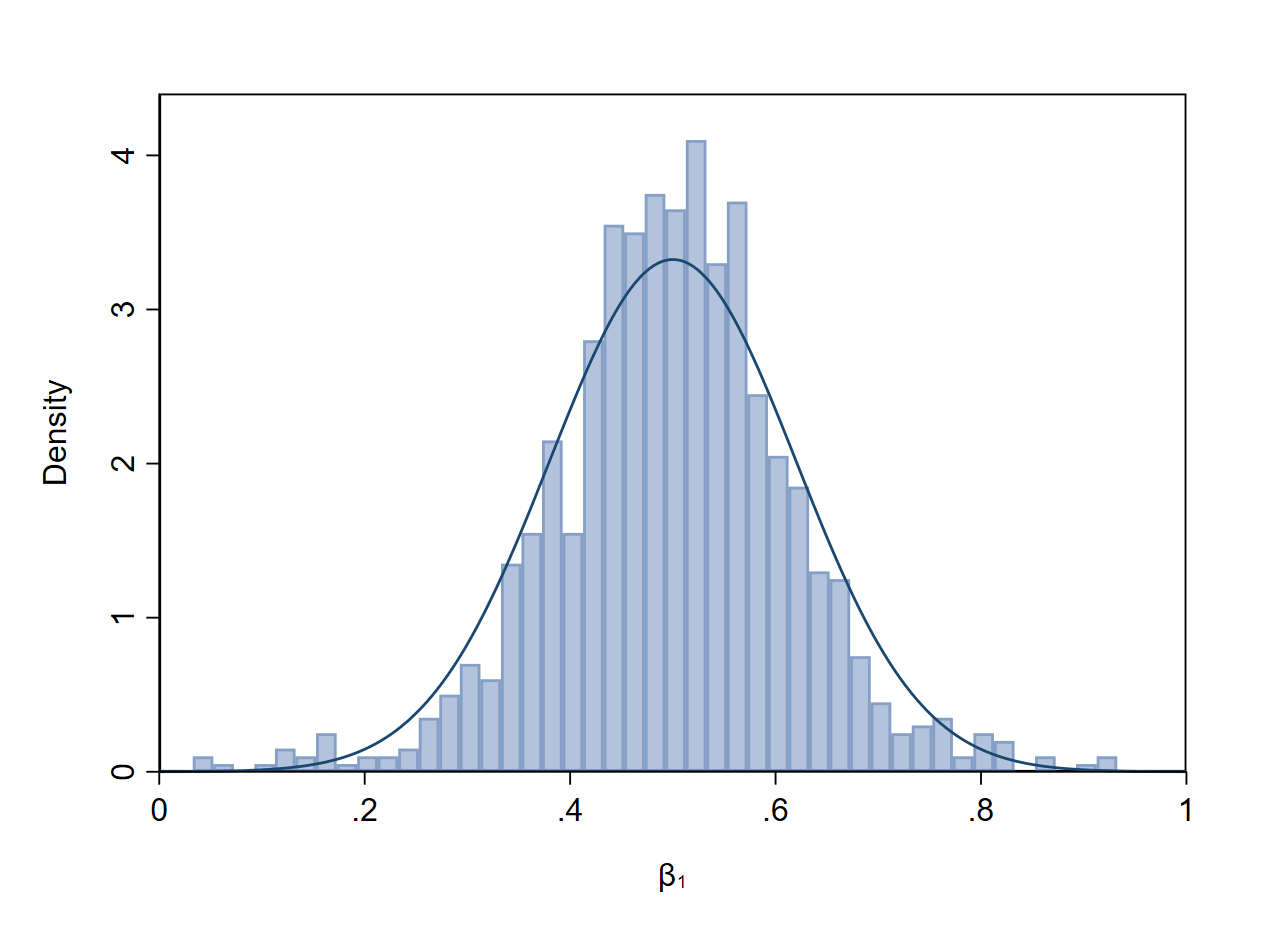
\includegraphics[width=1\textwidth]{figures/distribution_beta1_5}
		\caption{N=5}
		\label{fig:distribution beta1 N5}								
	\end{subfigure}\\
	\pause
	\begin{subfigure}[c]{0.49\textwidth}
		\centering
		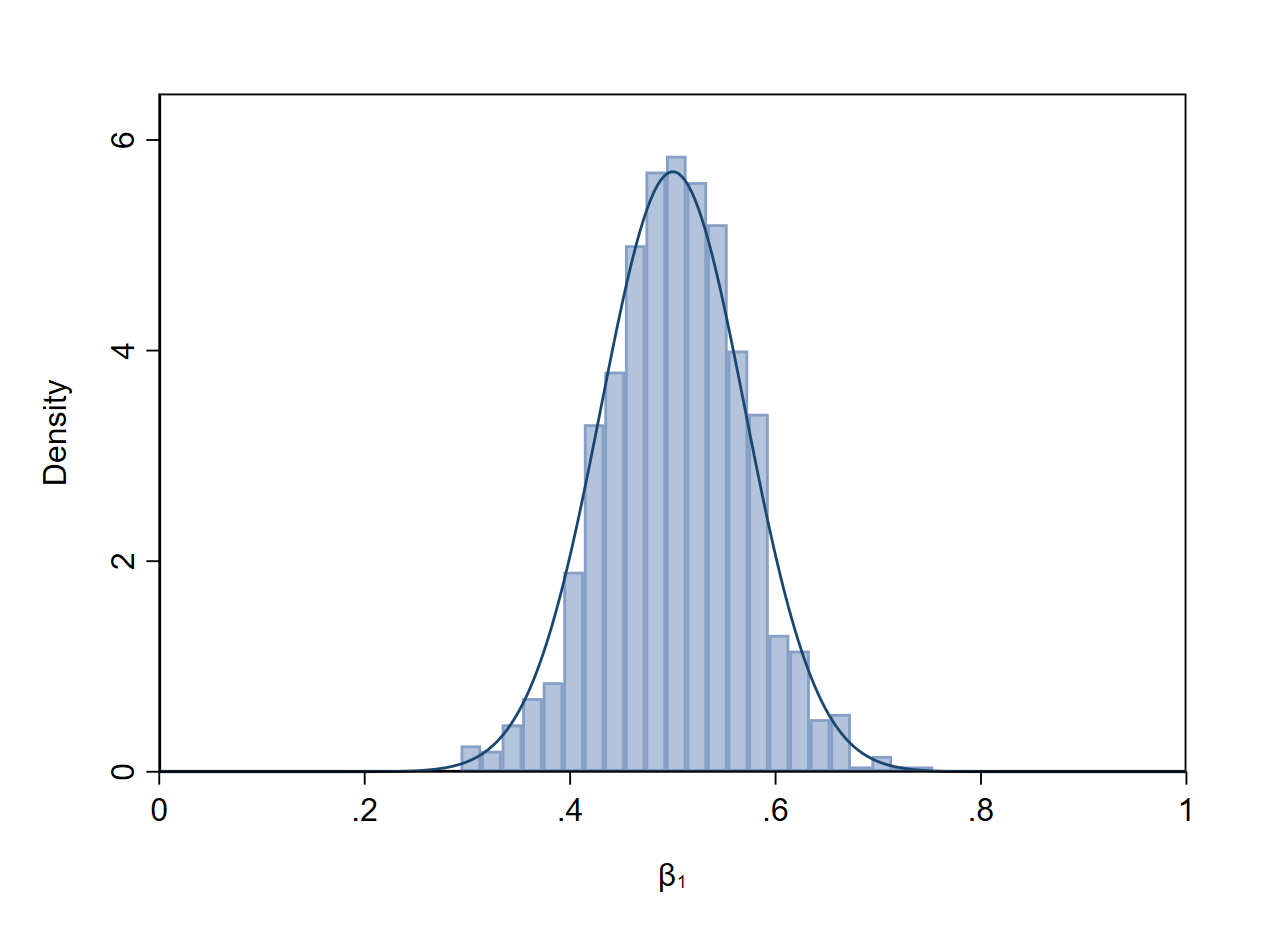
\includegraphics[width=1\textwidth]{figures/distribution_beta1_10}
		\caption{N=10}
		\label{fig:distribution beta1 N10}								
  \end{subfigure}
	\pause
	\begin{subfigure}[c]{0.49\textwidth}
		\centering
		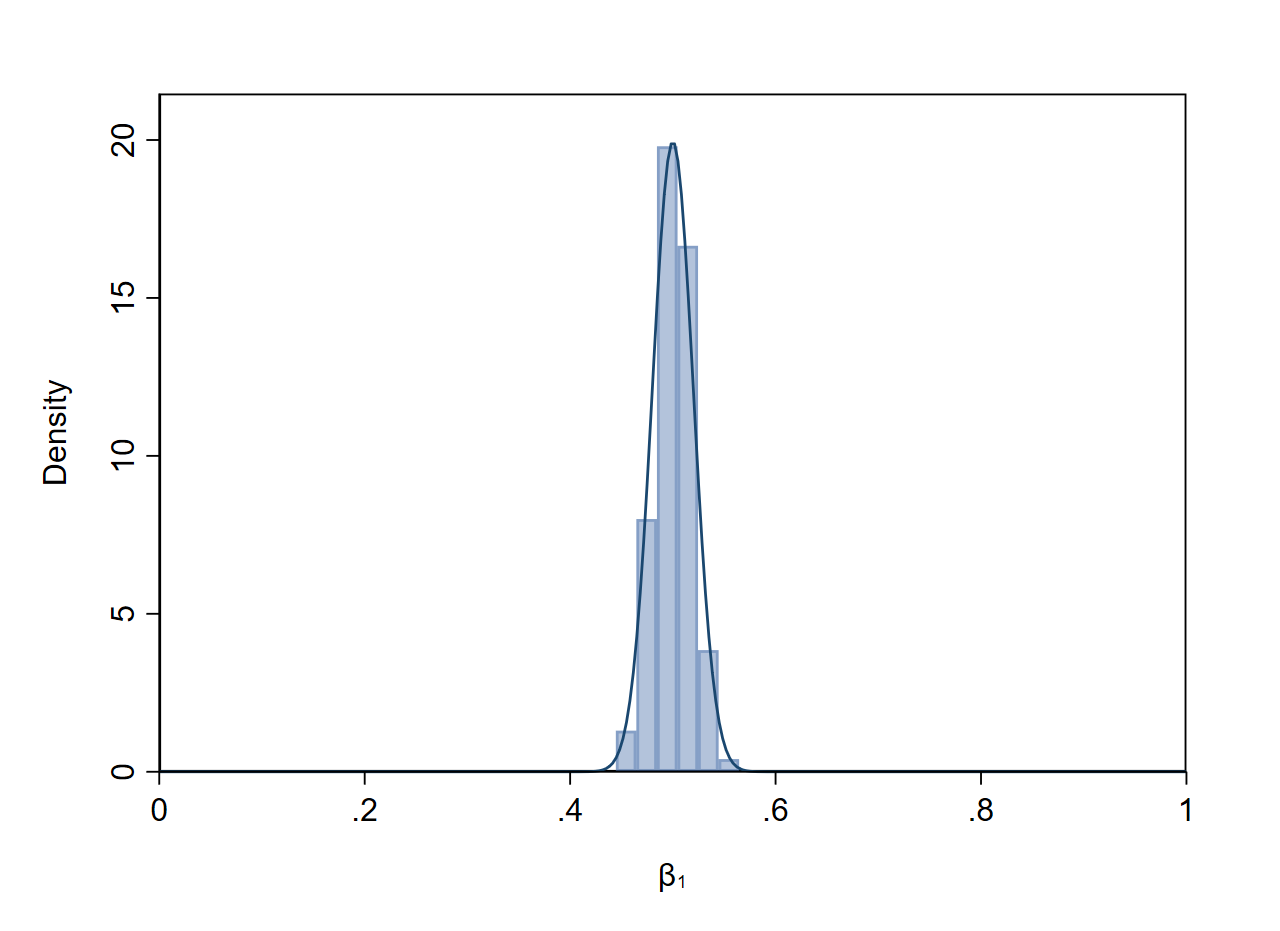
\includegraphics[width=1\textwidth]{figures/distribution_beta1_100}
		\caption{N=100}
		\label{fig:distribution beta1 N100}								
  \end{subfigure}
%\caption{Distribution of beta1}
\end{figure} 
%-------------------------------------------
\end{column}
\end{columns}

\end{frame}

\begin{frame}{How to Establish Asymptotic Properties of $\hat{\beta}_k$?}
%\beamerdefaultoverlayspecification{<+->}
\begin{columns}
\begin{column}{0.45\textwidth}
\small\pause
\textbf{Central Limit Theorem}\\\pause
As $N$ increases, the distribution of $\hat{\beta}_k$ becomes normal (starting from a $t$-distribution).\pause
\end{column}
\begin{column}{0.55\textwidth} 
%-------------------------------------------
\begin{figure}[htbp]
	\begin{subfigure}[c]{0.49\textwidth}
		\centering
		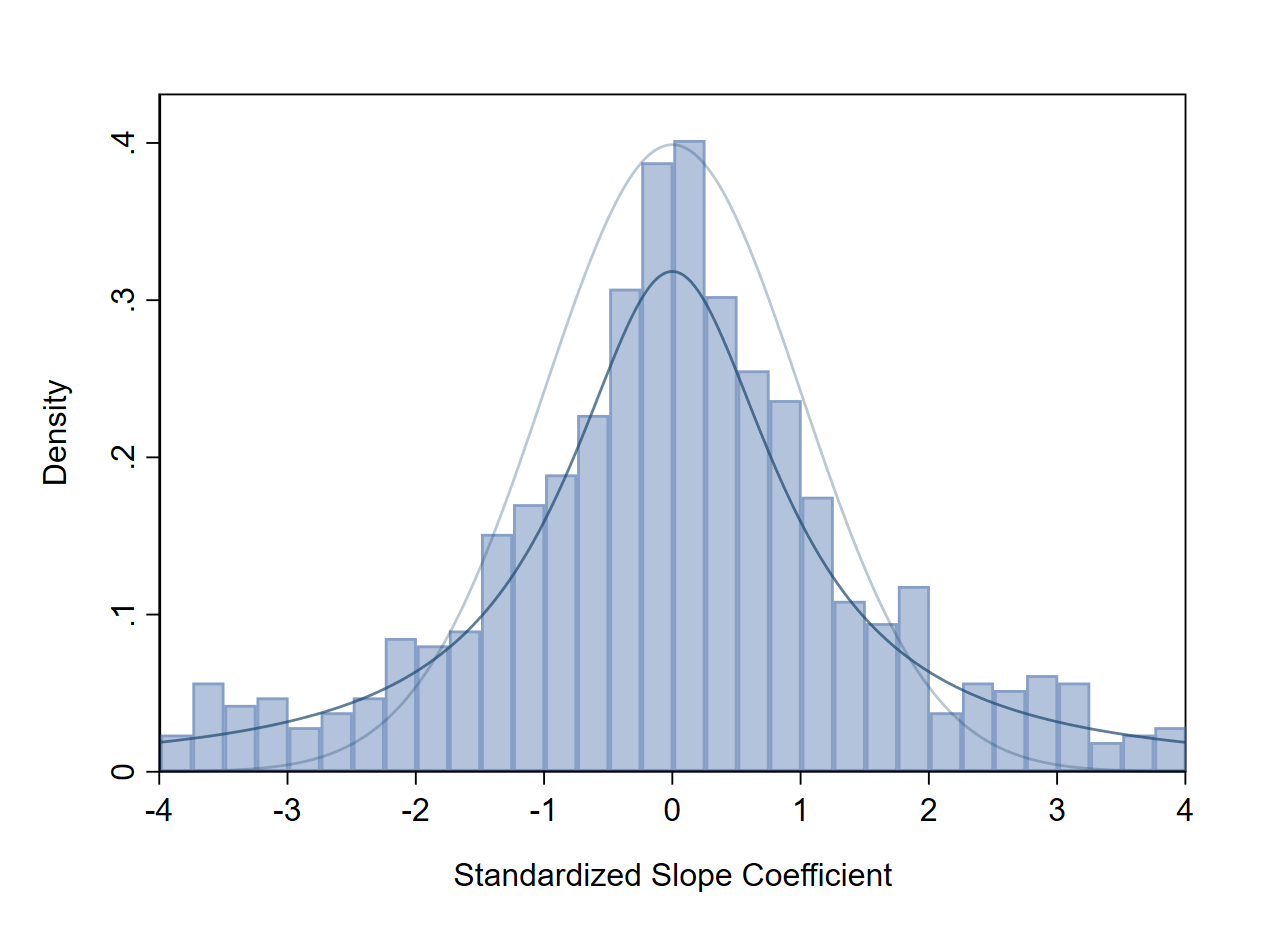
\includegraphics[width=1\textwidth]{figures/sampling_error_beta1_3}
		\caption{N=3}
    \label{fig:sampling error beta1 N3}
	\end{subfigure}%
	\pause
	\begin{subfigure}[c]{0.49\textwidth}
		\centering
		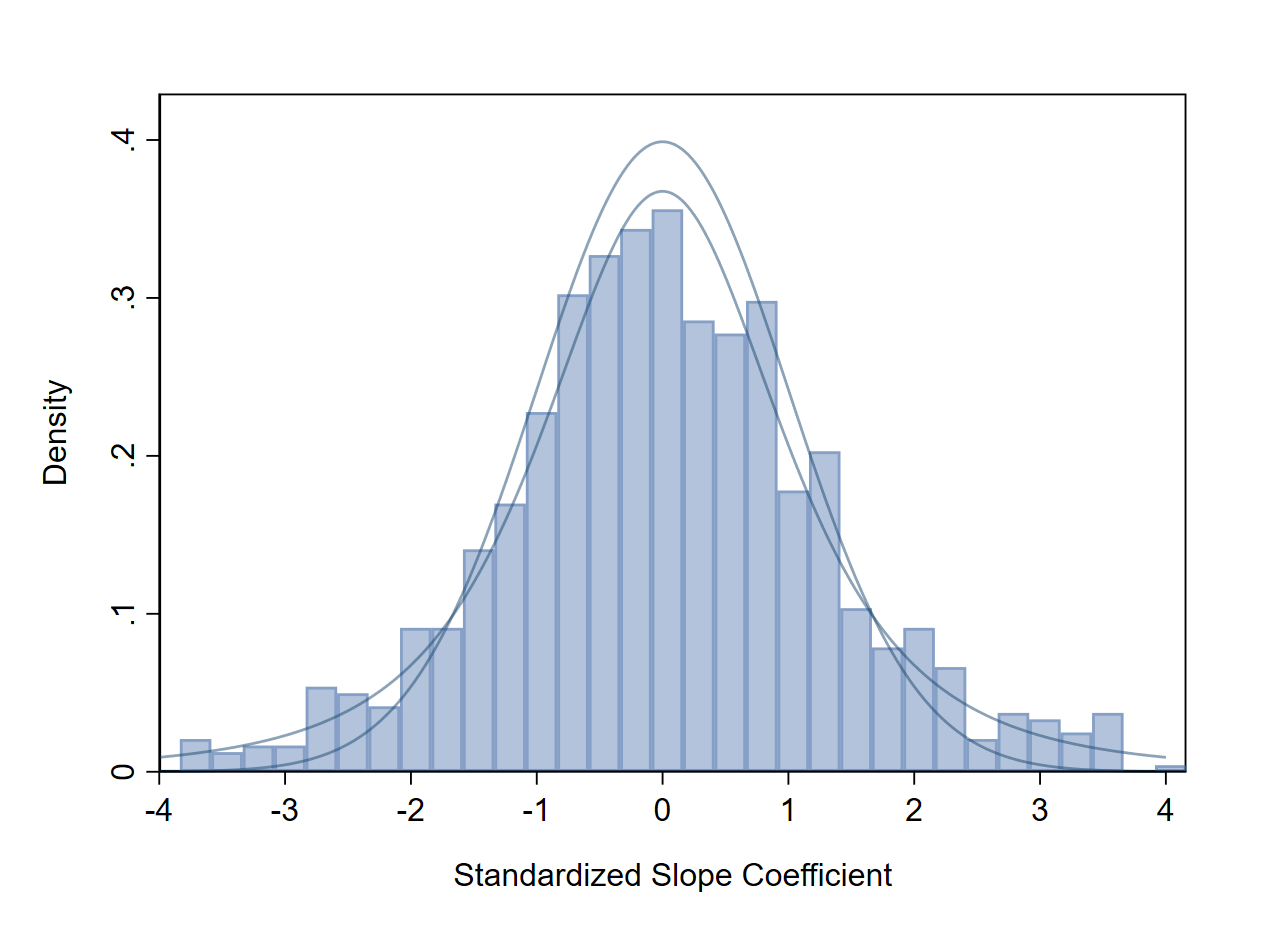
\includegraphics[width=1\textwidth]{figures/sampling_error_beta1_5}
		\caption{N=5}
		\label{fig:sampling error beta1 N5}								
	\end{subfigure}\\
	\pause
	\begin{subfigure}[c]{0.49\textwidth}
		\centering
		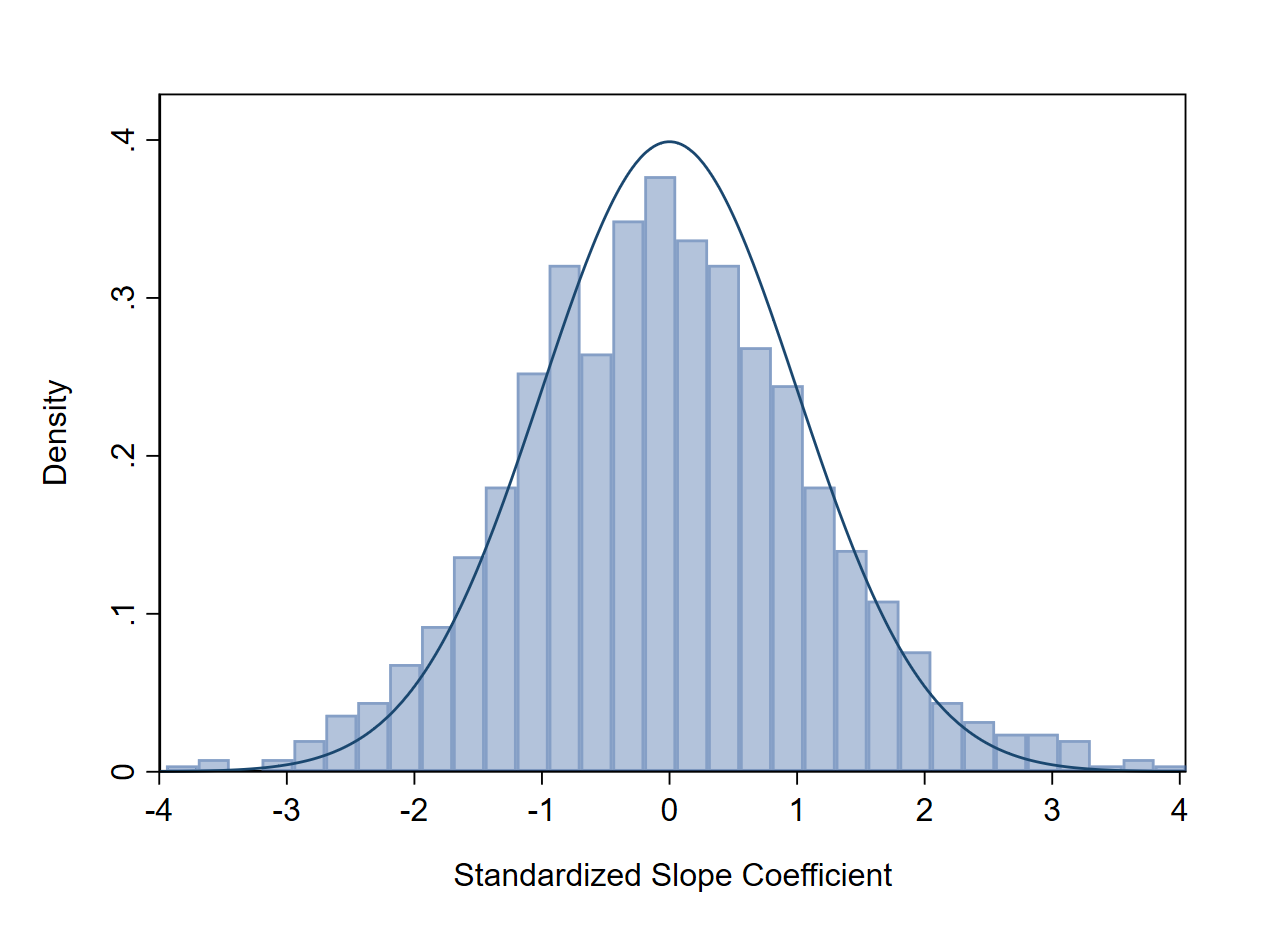
\includegraphics[width=1\textwidth]{figures/sampling_error_beta1_10}
		\caption{N=10}
		\label{fig:sampling error beta1 N10}								
  \end{subfigure}
	\pause
	\begin{subfigure}[c]{0.49\textwidth}
		\centering
		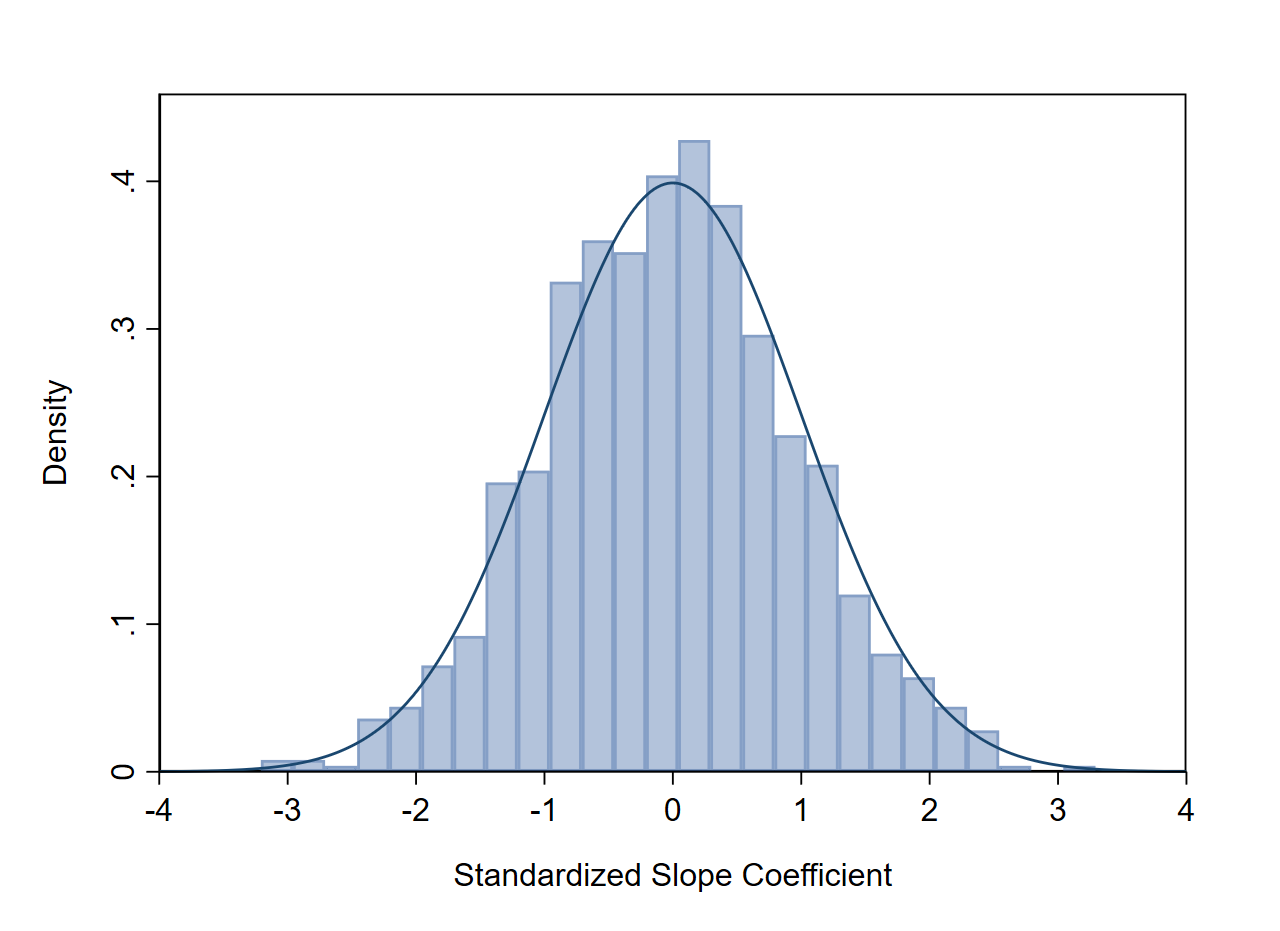
\includegraphics[width=1\textwidth]{figures/sampling_error_beta1_100}
		\caption{N=100}
		\label{fig:sampling error beta1 N100}								
  \end{subfigure}
%\caption{Distribution of beta1}
\end{figure} 
\end{column}
\end{columns}
\end{frame}




\begin{frame}{Consistency, Asymptotically Normality}
\beamerdefaultoverlayspecification{<+->}

Assuming LRM1, \pause LRM2, \pause LRM3d, \pause LRM4a or LRM4b, \pause and LRM5 \\\pause the following
properties can be established using law of large numbers and central limit theorem for large samples.\pause
\beX
\item The OLS estimator is \textbf{consistent}:\\\pause
$$plim \hat{\beta}_k = \beta_k.$$\pause
That is, for all $\varepsilon > 0$ $$\lim_{N\to\infty}\Pr\big(|\hat{\beta}_k-\beta_k| > \varepsilon\big) = 0.$$\pause
\item The OLS estimator is \textbf{asymptotically normally distributed}\pause
$$\sqrt{N} (\hat{\beta}_k-\beta_k) \overset{d}{\rightarrow} N(0,Avar(\hat{\beta}_k)\times N)$$\\(Avar means asymptotic variance)\pause
\item The OLS estimator is \textbf{approximately normally distributed}\pause
$$\hat{\beta}_k\overset{A}{\sim}N\left(\beta_k, Avar(\hat{\beta}_k)\right)$$
								
\eeX
\end{frame}


\begin{frame}{Efficiency and Asymptotic Variance}
\beamerdefaultoverlayspecification{<+->}

For the bivariate regression under LRM4a (homoskedasticity) it can be \textbf{consistently} estimated as
$$\widehat{Avar}(\hat{\beta}_1)=\frac{\hat{\sigma}^2}{\sum^{N}_{i=1}{(x_{i1}-\bar{x})^2}},$$\pause
with
$$\hat{\sigma}^2=\frac{\sum^{N}_{i=1}{\hat{u}^2_i}}{N-2}.$$
\pause
Under LRMb (heteroskedasticity), $Avar(\hat{\beta})$ can be \textbf{consistently} estimated as the \emph{robust} or \emph{Eicker-Huber-White} estimator.\pause\\[2ex] The robust variance estimator is calculated as\pause
$$\widehat{Avar}(\hat{\beta}_1)=\frac{\sum^{N}_{i=1}{\hat{u}^2_i(x_{i1}-\bar{x})^2}}{\left[\sum^{N}_{i=1}{(x_{i1}-\bar{x})^2}\right]}.$$\pause
Note: In practice we can almost never be sure that the errors are homoskedastic and should therefore always use robust standard errors.
\end{frame}



\begin{frame}{Sketch of Proof for Asymptotic Properties}
\beamerdefaultoverlayspecification{<+->}
\beX
\item The OLS estimator of $\hat\beta$ is consistent and asymptotic normal

Estimator $\hat\beta$ can be written as: $\hat\beta = \big(\tfrac{1}{N}X'X\big)^{-1}\tfrac{1}{N}X'y 
                  = \beta + \big(\tfrac{1}{N}X'X\big)^{-1}\tfrac{1}{N}X'u 
                  = \beta\; + \;\bigg(\frac{1}{N}\sum_{i=1}^N x_ix'_i\bigg)^{\!\!-1} \bigg(\frac{1}{N}\sum_{i=1}^N x_iu_i\bigg)$\pause\\[1ex]
We can use the law of large numbers to establish that 
: $\frac{1}{N}\sum_{i=1}^N x_ix'_i\ \xrightarrow{p}\ \operatorname{E}[x_ix_i']=\frac{Q_{xx}}{N}, \qquad 
        \frac{1}{N}\sum_{i=1}^N x_iu_i\ \xrightarrow{p}\ \operatorname{E}[x_iu_i]=0$\pause\\[1ex]
By Slutsky's theorem and continuous mapping theorem these results can be combined to establish consistency of estimator $\hat\beta$: $\hat\beta\ \xrightarrow{p}\ \beta + Q_{xx}^{-1}\cdot 0 = \beta$\pause\\[1ex]

The central limit theorem tells us that: $\frac{1}{\sqrt{N}}\sum_{i=1}^N x_iu_i\ \xrightarrow{d}\ \mathcal{N}\big(0,\,V\big),$ where  $V = \operatorname{Var}[x_iu_i] = \operatorname{E}[\,u_i^2x_ix'_i\,] = \operatorname{E}\big[\,\operatorname{E}[u_i^2|x_i]\;x_ix'_i\,\big] = \sigma^2 \frac{Q_{xx}}{N}$\pause\\[1ex]

Applying Slutsky's theorem again we'll have: $\sqrt{N}(\hat\beta-\beta) = \bigg(\frac{1}{N}\sum_{i=1}^N x_ix'_i\bigg)^{\!\!-1} \bigg(\frac{1}{\sqrt{N}}\sum_{i=1}^N x_iu_i\bigg)\ \xrightarrow{d}\ Q_{xx}^{-1}N\cdot\mathcal{N}\big(0, \sigma^2\frac{Q_{xx}}{N}\big) = \mathcal{N}\big(0,\sigma^2Q_{xx}^{-1}N\big)$
\qed
\eeX
\end{frame}

\begin{frame}{OLS Properties in the Small and in the Large}
\begin{table}
\centering
{
%\begin{tabular}{l*{5}{D{.}{.}{-1}}}
\begin{scriptsize}
\begin{tabular}{@{\extracolsep{4pt}}l*{6}{c}}
\toprule
Set of assumptions & (1) & (2) & (3) & (4) & (5) & (6)\\
\midrule
LRM1: linearity & \multicolumn{6}{c}{f\quad u\quad l\quad f\quad i\quad l\quad l\quad e\quad d} \\
LRM2: simple random sampling & \multicolumn{6}{c}{f\quad u\quad l\quad f\quad i\quad l\quad l\quad e\quad d} \\
LRM5: identifiability & \multicolumn{6}{c}{f\quad u\quad l\quad f\quad i\quad l\quad l\quad e\quad d}\\
LRM4: error variance & & & & & & \\
- LRM4a: homoskedastic & $\checkmark$ & $\checkmark$ & $\checkmark$ & $\times$ & $\times$ & $\times$\\
- LRM4b: heteroskedastic & $\times$ & $\times$ & $\times$ & $\checkmark$ & $\checkmark$ & $\checkmark$\\
LRM3: exogeneity& & & & & & \\
- LRM3a: normality & $\checkmark$ & $\times$ & $\times$ & $\checkmark$ & $\times$ & $\times$\\
- LRM3b: independent & $\checkmark$ & $\checkmark$ & $\times$ & $\times$ & $\times$ & $\times$\\
- LRM3c: mean indep. & $\checkmark$ & $\checkmark$ & $\checkmark$ & $\checkmark$ & $\checkmark$ & $\times$\\
- LRM3d: uncorrelated  & $\checkmark$ & $\checkmark$ & $\checkmark$ & $\checkmark$ & $\checkmark$ & $\checkmark$\\
\midrule
\multicolumn{7}{@{}l}{\emph{Small sample properties of $\hat{\beta}$}}\\
- unbiased & $\checkmark$ & $\checkmark$ & $\checkmark$ & $\checkmark$ & $\checkmark$ & $\times$\\
- normally distributed & $\checkmark$ & $\times$ & $\times$ & $\checkmark$ & $\times$ & $\times$\\
- efficient & $\checkmark$ & $\checkmark$ & $\checkmark$ & $\times$ & $\times$ & $\times$\\
%$t$-test, $F$-test & $\checkmark$ & $\times$ & $\times$ & $\times$ & $\times$ & $\times$\\
\midrule
\multicolumn{7}{@{}l}{\emph{Large sample properties of $\hat{\beta}$}}\\
- consistent & $\checkmark$ & $\checkmark$ & $\checkmark$ & $\checkmark$ & $\checkmark$ & $\checkmark$\\
- approx. normal & $\checkmark$ & $\checkmark$ & $\checkmark$ & $\checkmark$ & $\checkmark$ & $\checkmark$\\
- asymptotically efficient & $\checkmark$ & $\checkmark$ & $\checkmark$ & $\times$ & $\times$ & $\times$\\
%$z$-test, Wald test & $\checkmark$ & $\checkmark$ & $\checkmark$ & $\checkmark$* & $\checkmark$* & $\checkmark$*\\
\bottomrule
\end{tabular}
\end{scriptsize}
\beX
\begin{scriptsize}
\item \textit{Notes:} $\checkmark$ = fulfilled, $\times$ = violated%, * = corrected standard errors.
\end{scriptsize}
\eeX
}
%\caption{Assumptions and OLS Properties in the Small and in the Large. \label{tab:Summary}}

\end{table}
\end{frame}


\begin{frame}{Tests in Small Samples I}
\beamerdefaultoverlayspecification{<+->}

Assume LRM1, \pause LRM2, \pause LRM3a, \pause LRM4a, \pause and LRM5. \pause
A simple null hypotheses of the form $H_0: \beta_k = q$ is tested with the
\textbf{$t$-test}.

If the null hypotheses is true, the $t$-statistic\pause
 $$t=\frac{\hat{\beta}_k-q}{\widehat{se}(\hat{\beta}_k)}\sim t_{N-K-1}$$\pause
follows a $t$-distribution with $N-K-1$ degrees of freedom. The standard error is $\widehat{se}(\hat{\beta}_k) = \sqrt{\hat{V}(\hat{\beta}_k)}$.\\[2ex]
\pause
For example, to perform a two-sided test of $H_0$ against the alternative hypotheses $H_A: \beta_k \neq q$ on the 5\% significance level, we calculate the $t$-statistic and compare its absolute value to the 0.975-quantile of the $t$-distribution. With $N = 30$ and $K = 2$, $H_0$ is rejected if $|t| > 2.052$.
\end{frame}


\begin{frame}{Tests in Small Samples II}
\beamerdefaultoverlayspecification{<+->}

A null hypotheses of the form $H_0: r_{j1}\beta_1 + \ldots + r_{jK}\beta_K = q_j$, in matrix notation $H_0: R\beta = q$, with $J$ linear restrictions $j = 1\ldots J$ is jointly tested with the \textbf{$F$-test}.

\pause
If the null hypotheses is true, the $F$-statistic follows an $F$ distribution with $J$ numerator degrees of freedom and $N - K - 1$ denominator degrees of freedom:\pause
$$F = \frac{\left(R\hat{\beta}-q\right)'\left[R\hat{V}(\hat{\beta}|X)R'\right]^{-1}\left(R\hat{\beta}-q\right)}{J}\sim F_{J,N-K-1}.$$

\pause
For example, to perform a two-sided test of $H_0$ against the alternative hypotheses
$H_A: r_{j1}\beta_1 + \ldots + r_{jK}\beta_K \neq q_j$ for all $j$ at the 5\% significance level, we calculate the $F$-statistic and compare it to the 0.95-quantile of the $F$-distribution.\\[2ex] With $N = 30, K = 2$ and $J = 2$, $H_0$ is rejected if $F > 3.35$. We cannot perform two-sided $F$-tests because the $F$ distribution has one tail.

\end{frame}

\begin{frame}{Tests in Small Samples III}
\beamerdefaultoverlayspecification{<+->}

Only under homoskedasticity (LRM4a), the $F$-statistic can also be computed as\pause
$$F = \frac{(R^2-R^2_{\text{restricted}})/J}{(1-R^2)/(N-K-1)}\sim F_{J,N-K-1},$$\pause
where $R^2_{\text{restricted}}$ is estimated by restricted least squares which minimizes $SD(\beta)$ s.t. $r_{j1}\beta_1 +\ldots+r_{jK}\beta_K \neq q_j$ for all $j$.\\[2ex]

\pause

Exclusionary restrictions of the form $H_0: \beta_k = 0, \beta_m = 0, \ldots$ are a special case of $H_0: r_{j1}\beta_1 + \ldots + r_{jK}\beta_K = q_j$ for all $j$. In this case, restricted least squares is simply estimated as a regression were the explanatory variables $k, m, \ldots$ are excluded, e.g. a regression with a constant only.\\[2ex]
If the $F$ distribution has degrees of freedom (df) 1 as the numerator df, and $N-K-1$ as the denominator df, then it can be shown that $t^{2}=F(1,N-K-1)$.
\end{frame}



\begin{frame}{Confidence Intervals in Small Samples}
\beamerdefaultoverlayspecification{<+->}

Assuming LRM1, \pause LRM2, \pause LRM3a, \pause LRM4a, and \pause LRM5,\pause we can construct confidence intervals for a particular coefficient $\beta_k$.\pause The $(1-\alpha)$ confidence interval is given by

$$\left(\hat{\beta}_k-t_{(1-\alpha/2),(N-K-1)}\widehat{se}(\hat{\beta}_k), \hat{\beta}_k+t_{(1-\alpha/2),(N-K-1)}\widehat{se}(\hat{\beta}_k)\right),$$\pause
where $t_{(1-\alpha/2),(N-K-1)}$ is the $(1 - \alpha/2)$ quantile of the $t$-distribution with $(N-K-1)$ degrees of freedom. \pause For example, the 95\% confidence interval with $N=30$ and $K=2$ is $\left(\hat{\beta}_k-2.052\widehat{se}(\hat{\beta}_k), \hat{\beta}_k+2.052\widehat{se}(\hat{\beta}_k)\right)$.\\[2ex]

\end{frame}

\begin{frame}{Confidence Intervals in Small Samples}
\beamerdefaultoverlayspecification{<+->}


Recall: $\alpha$ is the maximum acceptable probability of a Type I error.

\begin{table}
\centering{
%\begin{tabular}{l*{5}{D{.}{.}{-1}}}
\begin{footnotesize}
\begin{tabular}{@{\extracolsep{4pt}}l*{3}{c}}
\toprule
Null hypothesis ($H_0$) & is valid (Innocent) & is invalid (Guilty)\\
\midrule
Reject $H_0$ & \textbf{Type I ($\alpha=0.05$) error} & Correct outcome\\[1ex]
I think he is guilty! & False positive & True positive\\
& Convicted! & Convicted!\\[2ex]
Don't reject $H_0$  & Correct outcome & \textbf{Type II ($\beta$) error}\\[1ex]
I think he is innocent! & True negative & False negative\\
& Freed! & Freed!\\
\bottomrule
\end{tabular}
\end{footnotesize}
}
\end{table}
\end{frame}




\begin{frame}{Asymptotic Tests}
\beamerdefaultoverlayspecification{<+->}

Assume LRM1, \pause LRM2, \pause LRM3d, \pause LRM4a or LRM4b, \pause and LRM5. \pause A simple null hypotheses of the form $H_0: \beta_k = q$ is tested with the \textbf{$z$-test}. If the null hypotheses is true, the $z$-statistic\pause
$$z =\frac{\hat{\beta}_k-q}{\widehat{se}(\hat{\beta}_k)}\overset{A}{\sim} N(0,1)$$
\pause
follows approximately the standard normal distribution. The standard error is $\widehat{se}(\hat{\beta}_k)=\sqrt{\widehat{Avar}(\hat{\beta}_k)}$.\\[2ex]

\pause For example, to perform a two sided test of $H_0$ against the alternative hypotheses $H_A: \beta_k \neq q$ on the 5\% significance level, we calculate the $z$-statistic and compare its absolute value to the 0.975-quantile of the standard normal distribution. $H_0$ is rejected if $|z|>1.96$.\\[2ex]

We talk about the Wald test later...
\end{frame}



\begin{frame}{Confidence Intervals in Large Samples}
\beamerdefaultoverlayspecification{<+->}

Assuming LRM1, \pause LRM2, \pause LRM3d, \pause LRM5, \pause and LRM4a or LRM4b, \pause we can construct confidence intervals for a particular coefficient $\beta_k$. \pause The $(1 - \alpha)$ confidence interval is given by

$$\left(\hat{\beta}_k-z_{(1-\alpha/2)}\widehat{se}(\hat{\beta}_k), \hat{\beta}_k+z_{(1-\alpha/2)}\widehat{se}(\hat{\beta}_k)\right)$$ \pause
where $z_{(1-\alpha/2)}$ is the $(1 - \alpha/2)$ quantile of the standard normal distribution.\\[2ex] \pause

For example, the 95\% confidence interval is $\left(\hat{\beta}_k-1.96\widehat{se}(\hat{\beta}_k), \hat{\beta}_k+1.96\widehat{se}(\hat{\beta}_k)\right)$.

\end{frame}



\begin{frame}{OLS Properties in the Small and in the Large}
\begin{table}
\centering
{
%\begin{tabular}{l*{5}{D{.}{.}{-1}}}
\begin{tiny}
\begin{tabular}{@{\extracolsep{4pt}}l*{6}{c}}
\toprule
Set of assumptions & (1) & (2) & (3) & (4) & (5) & (6)\\
\midrule
LRM1: linearity & \multicolumn{6}{c}{f\quad u\quad l\quad f\quad i\quad l\quad l\quad e\quad d} \\
LRM2: simple random sampling & \multicolumn{6}{c}{f\quad u\quad l\quad f\quad i\quad l\quad l\quad e\quad d} \\
LRM5: identifiability & \multicolumn{6}{c}{f\quad u\quad l\quad f\quad i\quad l\quad l\quad e\quad d}\\
LRM4: error variance & & & & & & \\
- LRM4a: homoskedastic & $\checkmark$ & $\checkmark$ & $\checkmark$ & $\times$ & $\times$ & $\times$\\
- LRM4b: heteroskedastic & $\times$ & $\times$ & $\times$ & $\checkmark$ & $\checkmark$ & $\checkmark$\\
LRM3: exogeneity& & & & & & \\
- LRM3a: normality & $\checkmark$ & $\times$ & $\times$ & $\checkmark$ & $\times$ & $\times$\\
- LRM3b: independent & $\checkmark$ & $\checkmark$ & $\times$ & $\times$ & $\times$ & $\times$\\
- LRM3c: mean indep. & $\checkmark$ & $\checkmark$ & $\checkmark$ & $\checkmark$ & $\checkmark$ & $\times$\\
- LRM3d: uncorrelated  & $\checkmark$ & $\checkmark$ & $\checkmark$ & $\checkmark$ & $\checkmark$ & $\checkmark$\\
\midrule
\multicolumn{7}{@{}l}{\emph{Small sample properties of $\hat{\beta}$}}\\
- unbiased & $\checkmark$ & $\checkmark$ & $\checkmark$ & $\checkmark$ & $\checkmark$ & $\times$\\
- normally distributed & $\checkmark$ & $\times$ & $\times$ & $\checkmark$ & $\times$ & $\times$\\
- efficient & $\checkmark$ & $\checkmark$ & $\checkmark$ & $\times$ & $\times$ & $\times$\\
$t$-test, $F$-test & $\checkmark$ & $\times$ & $\times$ & $\times$ & $\times$ & $\times$\\
\midrule
\multicolumn{7}{@{}l}{\emph{Large sample properties of $\hat{\beta}$}}\\
- consistent & $\checkmark$ & $\checkmark$ & $\checkmark$ & $\checkmark$ & $\checkmark$ & $\checkmark$\\
- approx. normal & $\checkmark$ & $\checkmark$ & $\checkmark$ & $\checkmark$ & $\checkmark$ & $\checkmark$\\
- asymptotically efficient & $\checkmark$ & $\checkmark$ & $\checkmark$ & $\times$ & $\times$ & $\times$\\
$z$-test, Wald test & $\checkmark$ & $\checkmark$ & $\checkmark$ & $\checkmark$* & $\checkmark$* & $\checkmark$*\\
\bottomrule
\end{tabular}
\end{tiny}
\beX
\begin{tiny}
\item \textit{Notes:} $\checkmark$ = fulfilled, $\times$ = violated, * = corrected standard errors.
\end{tiny}
\eeX
}
%\caption{Assumptions and OLS Properties in the Small and in the Large. \label{tab:Summary}}

\end{table}
\end{frame}



\section{Politically Connected Firms: Causality or Correlation?}

 %--------------------------------------------------- Slide --
\begin{frame}
	\frametitle{Content}
	\tableofcontents[%
 		currentsection, % causes all sections but the current to be shown in a semi-transparent way.
 		%currentsubsection, % causes all subsections but the current subsection in the current section to ...
 		%hideallsubsections, % causes all subsections to be hidden.
 		%hideothersubsections, % causes the subsections of sections other than the current one to be hidden.
 		%part=, % part number causes the table of contents of part part number to be shown
 		%pausesections, % causes a \pause command to be issued before each section. This is useful if you
 		%pausesubsections, %  causes a \pause command to be issued before each subsection.
 		%sections={ overlay specification },
	]

\end{frame}


\begin{frame}{Arguments \textbf{For} Causality of Effect}
\beamerdefaultoverlayspecification{<+->}
\begin{figure}[t]
	\centering
		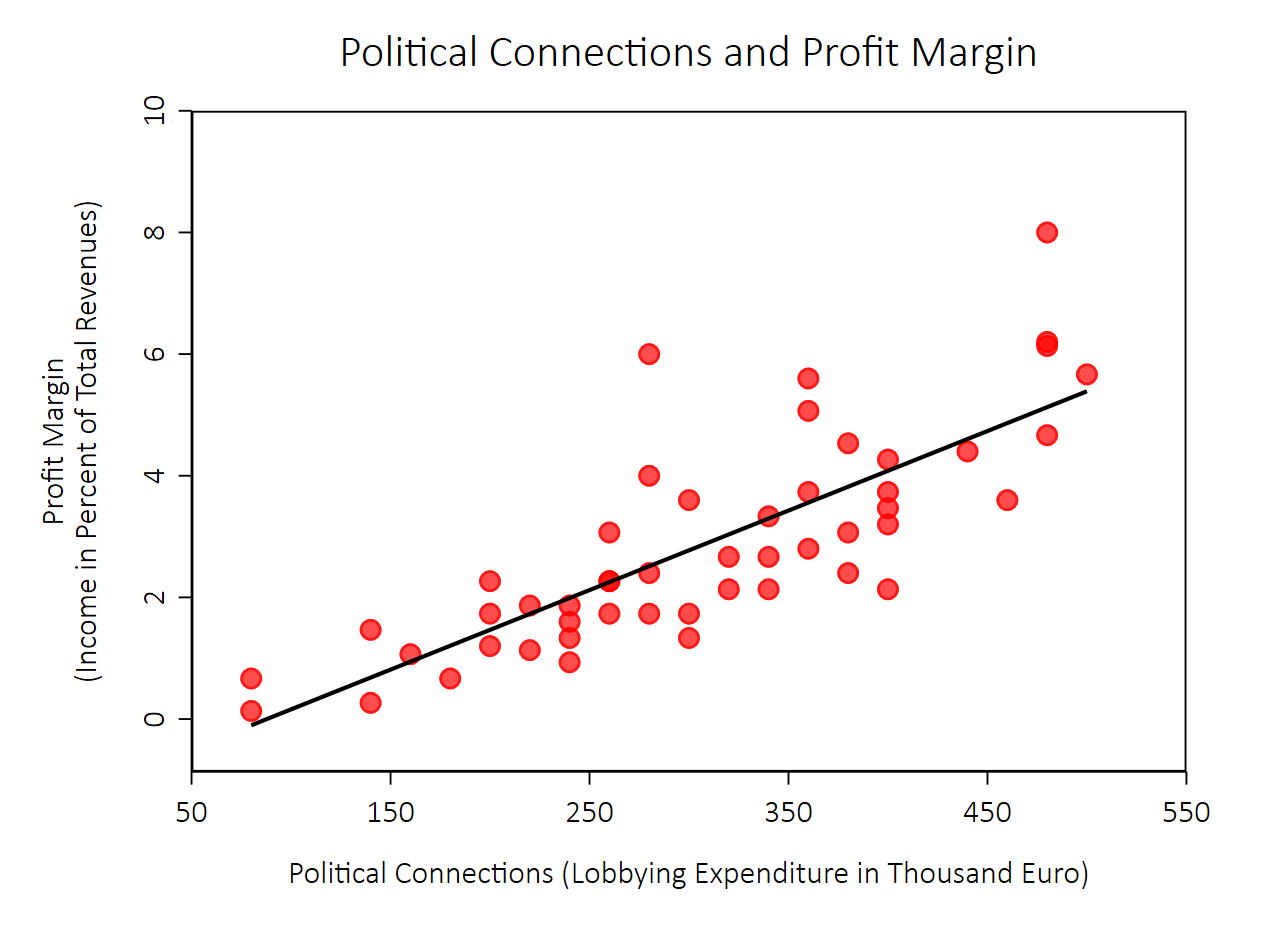
\includegraphics[height=.50\textheight]{figures/politicallyconnected4}
\end{figure}
\pause
Econometric methods need to address concerns, including:\\
\begin{itemize}
 \item \textbf{Misspecification:} Results robust to different functional forms
 \item \textbf{Errors-in-variables:} little concern with administrative data
 \item \textbf{External validity:} Similar effect found in independent studies.\\[3ex]
\end{itemize}

\end{frame}


\begin{frame}{Arguments \textbf{Against} Causality of Effect}
\beamerdefaultoverlayspecification{<+->}
\begin{itemize}
\item \textbf{Omitted variable bias:}\\ e.g., business acumen\\
$\rightarrow$ Panel data models
\item \textbf{Sample selection bias:}\\ lobbying expenditures only observed if in transparency register.\\
$\rightarrow$ Selection correction models
\item \textbf{Simultaneous causality:}\\
\begin{itemize}
	\item profits may be higher because of political connections
  \item firms may become connected because of their high profits\\[2ex]
%	\item is there a revolving door between politics and business?
\end{itemize}
\pause
\emph{All of those concerns may be addressed with}\\ $\rightarrow$\emph{instrumental variable models. What would be a good instrument/experiment?}
\end{itemize}

\end{frame}


%\setlength{\bibsep}{0pt}
%\def\newblock{References} 
%{\footnotesize
%\bibliography{bib}}


\begin{frame}[t,allowframebreaks
]\nocite{*}
\frametitle{References}
\small
\bibliography{bib}
\end{frame}




\end{document}
